\documentclass[10pt, landscape]{article}
\usepackage[scaled=0.92]{helvet}
\usepackage{multicol}
\usepackage{calc}
\usepackage{ifthen}
\usepackage[landscape]{geometry}
%\usepackage{hyperref}

\usepackage{newtxtext} 

%for strikeout
\usepackage{ulem}

%For editing parbox
\usepackage[table]{xcolor}
%For editing itemise margins, reduce iterm separaion and list separation
\usepackage{enumitem}
% For math
\usepackage{amsmath,amsthm,amsfonts,amssymb}

%For pictures / figures
\usepackage{color,graphicx,overpic}
\graphicspath{ {./images/} }

%\usepackage{newtxtext} 
%\usepackage{amssymb}
%\usepackage[table]{xcolor}
%\usepackage{vwcol}
%\usepackage{tikz}
%\usepackage{wrapfig}
%\usepackage{makecell}

\pdfinfo{
  /Title (CS2107-notes.pdf)
  /Creator (Ger Teck)
  /Author (Ger Teck)
  /Subject ()
  /Keywords (tex)}

%% Margins for PAPER

% This sets page margins to .5 inch if using letter paper, and to 1cm
% if using A4 paper. (This probably isn't strictly necessary.)
% If using another size paper, use default 1cm margins.
\ifthenelse{\lengthtest { \paperwidth = 11in}}
	{ \geometry{top=.3in,left=.3in,right=.3in,bottom=.3in} }
	{\ifthenelse{ \lengthtest{ \paperwidth = 297mm}}
		{\geometry{top=0.5cm,left=0.5cm,right=0.5cm,bottom=0.5cm} }
		{\geometry{top=0.5cm,left=0.5cm,right=0.5cm,bottom=0.5cm} }
	}

% Turn off header and footer
\pagestyle{empty}
% for tight centres (less spacing)
\newenvironment{tightcenter}{%
  \setlength\topsep{0.5pt}
  \setlength\parskip{0.5pt}
  \begin{center}
}{%
  \end{center}
}

% Redefine section commands to use less space
\makeatletter
\renewcommand{\section}{\@startsection{section}{1}{0mm}%
                                {-1ex plus -.5ex minus -.2ex}%
                                {0.5ex plus .2ex}%x
                                {\normalfont\large\bfseries}}
\renewcommand{\subsection}{\@startsection{subsection}{2}{0mm}%
                                {-1explus -.5ex minus -.2ex}%
                                {0.5ex plus .2ex}%
                                {\normalfont\normalsize\bfseries}}
\renewcommand{\subsubsection}{\@startsection{subsubsection}{3}{0mm}%
                                {-1ex plus -.5ex minus -.2ex}%
                                {1ex plus .2ex}%
                                {\normalfont\small\bfseries}}
% change font
%\renewcommand{\familydefault}{\sfdefault}
%\renewcommand\rmdefault{\sfdefault}
\linespread{1.05}

\makeatother

% Define BibTeX command
\def\BibTeX{{\rm B\kern-.05em{\sc i\kern-.025em b}\kern-.08em
    T\kern-.1667em\lower.7ex\hbox{E}\kern-.125emX}}

% Don't print section numbers
\setcounter{secnumdepth}{0}

\setlength{\parindent}{0pt}
\setlength{\parskip}{0pt plus 0.5ex}

%% this changes all items (enumerate and itemize, reduce margins) ITEMIZE SEPARATION HERE
\setlength{\leftmargini}{0.5cm}
\setlength{\leftmarginii}{0.5cm}
\setlist[itemize,1]{leftmargin=2mm,labelindent=1mm,labelsep=1mm, itemsep = 0mm}
\setlist[itemize,2]{leftmargin=4mm,labelindent=1mm,labelsep=1mm, itemsep = 0mm}

%itemsep = 0mm
%\setlist{nosep}

% -------------------------------------------------------------------------------

% START OF DOCUMENT HERE

\begin{document}
\raggedright
\footnotesize
\begin{multicols*}{3}

% multicol parameters
% These lengths are set only within the two main columns
%\setlength{\columnseprule}{0.25pt}
\setlength{\premulticols}{1pt}
\setlength{\postmulticols}{1pt}
\setlength{\multicolsep}{1pt}
\setlength{\columnsep}{2pt}

%% DOCUMENT NAME HERE
\begin{center}
     \Large{\textbf{CS2107 Introduction to \\
     				 Information Security}} \\
\end{center}
AY23/24 Sem 2, github.com/gerteck


\section{0. Introduction}
CS2107: Introductory module, illustrates fundamentals of how systems fail due to malicious activities and how they can be protected. 

\textbf{Lecture Notes notation}
\begin{itemize}
\item \textbf{Textbook:} Security in Computing (5th ed). Prentice Hall. Reference [PFx.y] refer to chapter x section y of this book.
\item Links with ``read'': Part of lecture, required. 
\item Links with ``see'': Optional good to browse references.
\end{itemize}

\subsection{Internet Security Threat Report Exc. Summary}
Persistent threats are threats that often operate within the shadows, outside of attention focused. 
\begin{itemize}
\item Highly targeted, often use combination of social engineering and software vulnerabilities to establish footholds within the targeted enterprise.
\item Network protection not enough to mitigate threats, comprehensive monitoring program required to scan all internal and external network traffic. Identifying, securing data is also key to protecting assets.
\item Recent attack types: Formjacking, Ransomware, Living off the Land (LotL), 
\end{itemize}


\subsection{Introduction to Computer/Info Security}
Systems may fail due to operator mistakes, hardware failures, poor implementation etc. Many systems robust against typical noise. Security is about intentional failures inflicted by deliberate human actions. \\
\textbf{Security Definitions:} C-I-A triad
\begin{itemize}
\item \textbf{Confidentiality}: Prevention of unauthorized disclosure of information.
\item \textbf{Integrity}: Prevention of unauthorized modification of info / processes.
\item \textbf{Availability}: Prevention of unauthorized withholding of info / resources.
\item Other requirements may include (Confidentiality: anonymity, covert channel), (Integrity: Non-repudiation (digital signature)), (Other: Accountability, traitor-tracing (printout w hidden watermark)) etc.
\item Importance of understanding security requirements before adopting mechanisms. Do not adopt mismatched protection mechanisms.
\end{itemize}

\subsubsection{Difficulties in achieving Security}
\begin{itemize}
\item \textbf{Security not considered} (in early design stage). \\
Lack of adversarial thinking in design / trade-off in security with ease-of-use, performance / cost.
\item Difficult to formulate requirements /design / implementation bugs. 
\item Difficult to operate/manage (Human error). \\
\item \textbf{Known Vulnerabilities: CVE (Common vulnerabilities \& Exposures}. Repository of discovered vulnerabilities. Significant portion considered "implementation bugs".
\item \textbf{Zero-day Vulnerabilities}: Unpublished vulnerabilities. If attackers deploy attacks on zero-day v., victims have "zero-day" to react. Not easy to get.
\end{itemize} 


\section{1. Encryption}

% To update:
\textbf{Key Summary \& Takeaways}
\begin{itemize}
\item \textbf{Encryption designed for confidentiality.} (Not necessarily integrity).
\item Formulate attack scenario by defining attacks it can prevent. 
\item Notions of "Oracle": Encryption, Decryption, Padding Oracle.
\item \textbf{Key strength}: Quantifying security by equivalence of best-known attack to exhaustive search.
\item No known efficient attacks on modern schemes under "original" threat models, but there are pitfalls. Such as implementation error (wrong mode, wrong random source, mishandle of IV), side channel attack, implicity require integrity, padding oracle attack.
\item Design of various symmetric key encryption schemes:
	\begin{itemize}
	\item One-time pad, stream cipher (xor'ing with "pseudo-random" string)
	\item Block cipher (mode of operations: CBC, ECB, CTR, GCM)
	\end{itemize}
\item \textbf{Crucial role of IV}. (Need randomness for indistinguishability). Make encryption probabilistic, how it is deployed, why it is important.
\end{itemize}

\subsubsection{Definitions}
\begin{itemize}
\item \textbf{Symmetric Key Encryption Scheme}: Two algorithms: encryption and decryption. Meets correctness property, and must be secure.
\item \textbf{Correctness:} $(D_k (E_k (x) ) = x )$. \textbf{Security}: Informally, "difficult" to derive useful info of the key k, and plaintext x. Ciphertext resemble random sequence of bytes.
\item \textbf{Cryptography}: Study of techniques in securing communication in present of adversaries with access. Encryption just a primitive (other includes crypto hash, digital signature etc. Common placeholders: Alice, Bob, Eve ("eavesdroppper"), Mallory (malicious, modify message), etc.
\end{itemize}

\subsubsection{Attack Model}
\textit{Aka: Threat / Adversary / Security Model, Attack Scenario.} \\
Measuring \textbf{security of a system}: Through attack classes it can prevent. Secure w.r.t these classes of attacks. Attack models are application-dependent. Attack models described by:
\begin{itemize}
\item Attacker's knowledge (info / service exposed) and computing resources
\item Attacker's goal
\end{itemize}
\textbf{Types of information we assume access to:} (Access to info can be formulated to accesses to an \textbf{"Oracle"}).
\begin{itemize}
\item \textbf{Ciphertext only attack:} Adversary given collection of ciphertext c. May know some properties 
of the plaintext, for e.g. the plaintext is an English sentence. (adv. can’t choose plaintext).
\item \textbf{Known plaintext attack:} Adversary given collection of plaintext m and corresponding ciphertext c. (adv. can’t choose plaintext.)
\item \textbf{Chosen plaintext attack (CPA):} Access to blackbox (i.e. the oracle). \\
Can choose, feed any plaintext m, obtain corresponding ciphertext c (all encrypt with the same key), reasonable large number of times. Can see ciphertext and choose next input.  \textit{(black-box called encryption oracle).}
\item \textbf{Chosen ciphertext attack (CCA2)}: Same as chosen plaintext attack, but adv. chooses ciphertext and blackbox outputs plaintext. \textit{black-box called decryption oracle}. \\
\textbf{Note}: (strange to assume attacker has power to decrypt, but good reason is that in some practical scenario, attacker does have some but not full decryption capability, e.g. \textit{padding oracle}. To cater for all scenarios, in formulation and design of encryption, we consider oracle with full decryption capability.)
\end{itemize}

\subsubsection{Adversary's Goals}
\begin{itemize}
\item \textbf{Total Break}: Attacker wants to find the key.
\item \textbf{Partial Break}: Few definitions, e.g. decrypt ciphertext, determine coarse information about plaintext, etc.
\item \textbf{Indistinguishability (IND)}: ) Attacker may satisfy with distinguishability of ciphertext: with some “non-negligible” probability more than ½, the attacker is able to distinguish the ciphertexts of a given plaintext (say, “Y”) from the ciphertext of another given plaintext (say, “N”). (Equivalently, unable to distinguish the ciphertext and a randomly sequence).
\item \textbf{Note}: total break most difficult goal, since achieves all. Distinguishability weakest goal, design cryptosystem preventing weakest goal.
\end{itemize}

\section{Classicial Ciphers (Symmetric)}

\subsection{1. Substitution Cipher}
\begin{itemize}
\item \textbf{Plaintext, ciphertext}: String over a set of symbols U.
\item \textbf{Key}: Subsitution table S, 1-1 onto function from U to U.
\item \textbf{Key space}: Set of all possible keys (e.g. 27). \textbf{Space Size} is total number of possible keys (factorial, 27!). \textbf{Key Size} is number of bits required to represent a key. (log 2 (27!), since 27! unique) 
\item \textbf{Exhaustive Search (Brute-force): Can be infeasible in worst case}
\item \textbf{Known-plaintext-attack}: Access to pairs of ciphertext and corresponding plaintexts: \textit{Sub. cipher “not secure / totally broken under known plaintext attack”}. (Possible in practice, e.g. certain words in header of email "From, Subject", protocols bytes fixed header information etc.)
\item \textbf{Ciphertext only attack}: Vulnerable to frequency analysis attack, when plaintexts English sentences.
\end{itemize}

\subsection{2. Permutation Cipher (aka transposition cipher)}
\begin{itemize}
\item Groups plaintext into blocks of $t$ characters, applies secret permutation (1-1 onto function). Fails miserably on known-plaintext attack.
\centerline{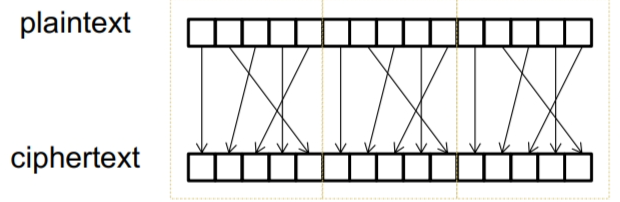
\includegraphics[width=0.4\linewidth]{permutationCipher}}
\end{itemize}

\begin{itemize}
\item S \& P cipher not secure, performing substitution multiple times no use. However, by interlacing them (S\&P), attacks become more difficult. Many modern encryption scheme (e.g. AES) designed using rounds of S \& P.
\end{itemize}

\subsection{Terminology}
\begin{itemize}
\item \textbf{Cryptosystem}: A system for encryption and decryption.
\item \textbf{Plaintext}: Original form of message.
\item \textbf{Ciphertext}: Encrypted form of message.
\item \textbf{Perfect Secrecy}: A cryptosystem has perfect secrecy if for any distribution $X$, for all $x, y$:
\centerline{$Pr ( X=x | Y=y ) = Pr (X =x) $}.
\item For any ciphertext $y$ and plaintext $x$, the chances attacker correctly predicts x before knowing y, and after knowing y, are the 
same.
\item \textbf{Work Factor}: Difficulty of breaking an encryption (Amount of effort necessary). \\
- (E.g. determine time it would take to test single password, multiply by total possible passwords).
\end{itemize}

\null \null \null \null


\columnbreak

\subsection{3. One Time Pad}
One-time pad (OTP) is an encryption technique that requires the use of a single-use pre-shared key that is larger than or equal to the size of the message being sent. 
\begin{itemize}
\item Plaintext is paired with a random secret key (known as one-time pad). 
\item Each bit or character of the plaintext encrypted by combining it with corresponding bit/character from pad using modular addition.[1]
\end{itemize}
\centerline{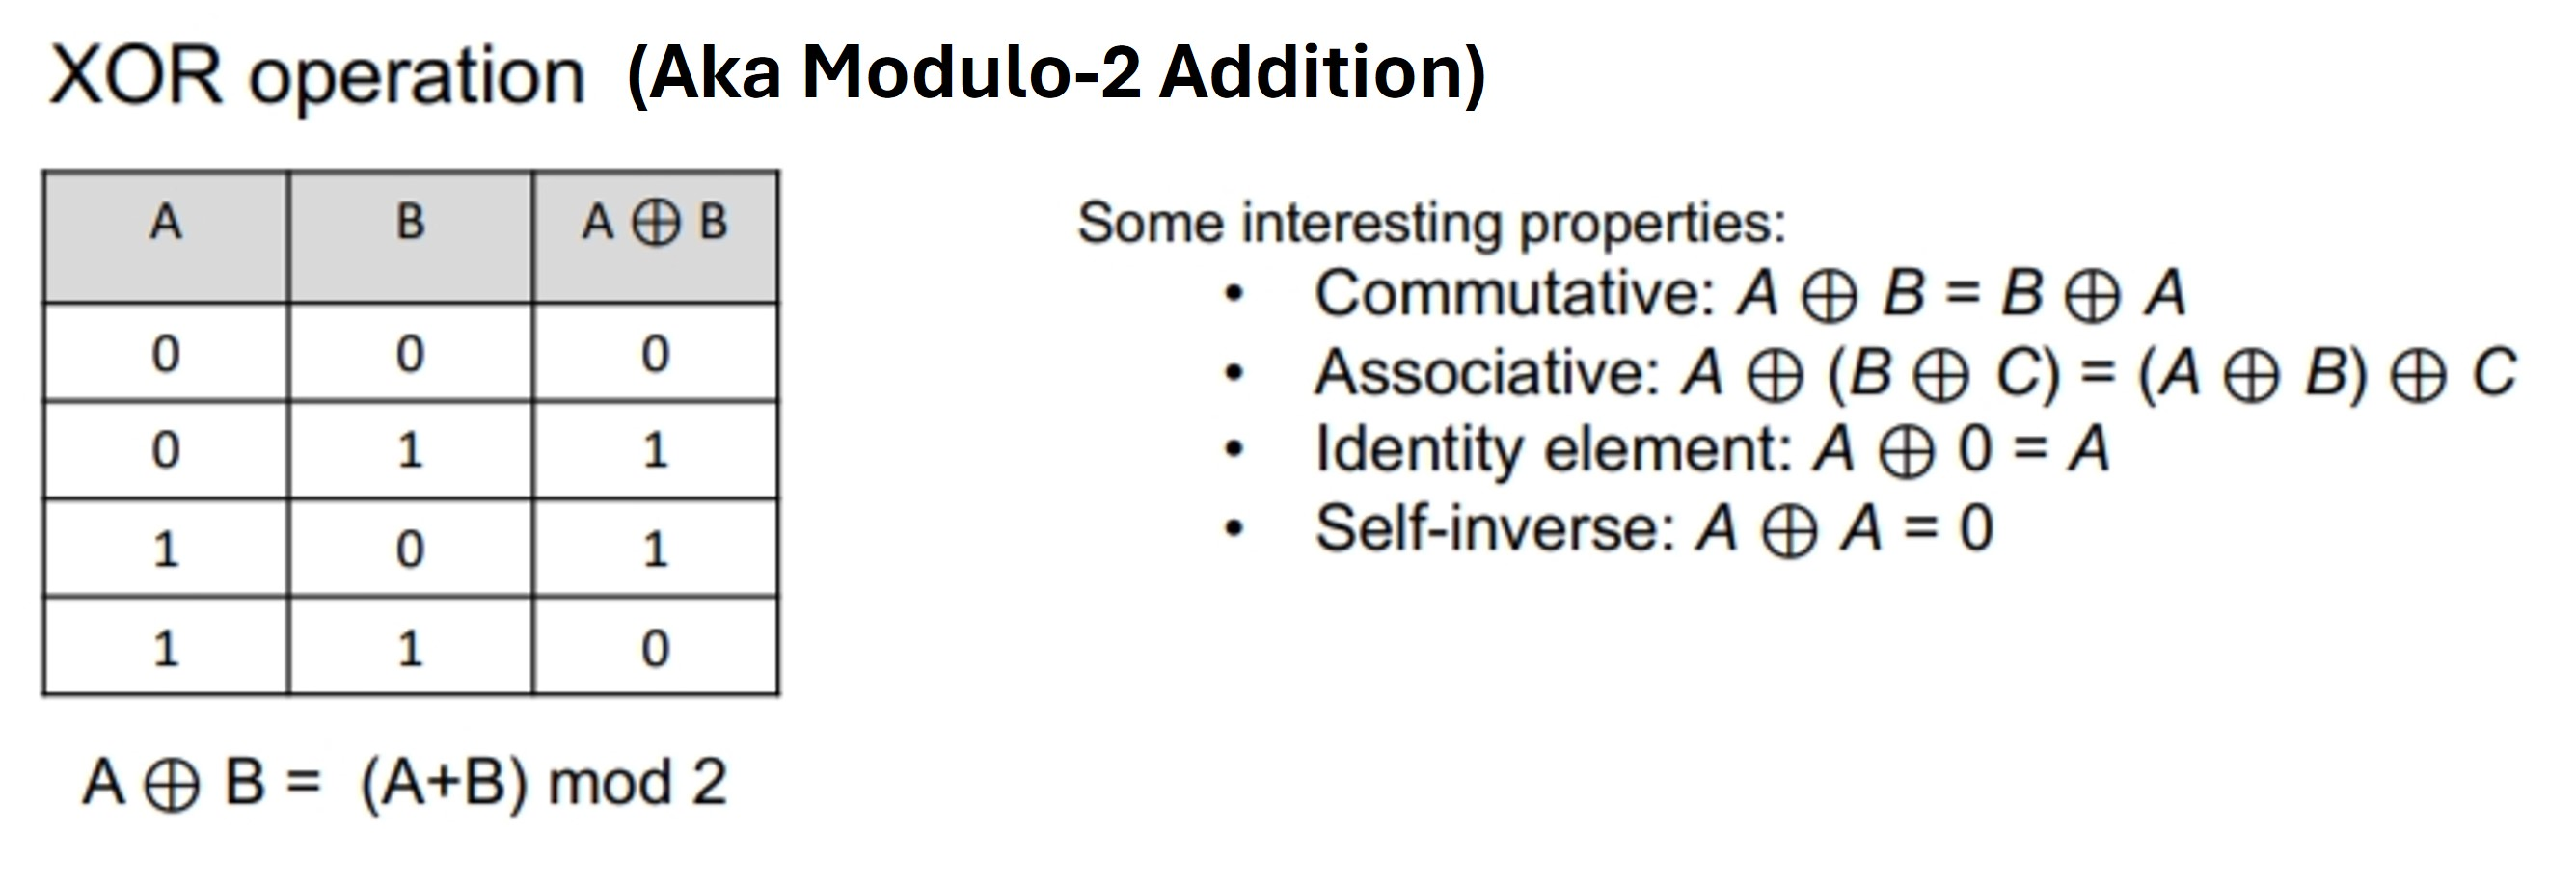
\includegraphics[width=0.4\linewidth]{XOR}}
\centerline{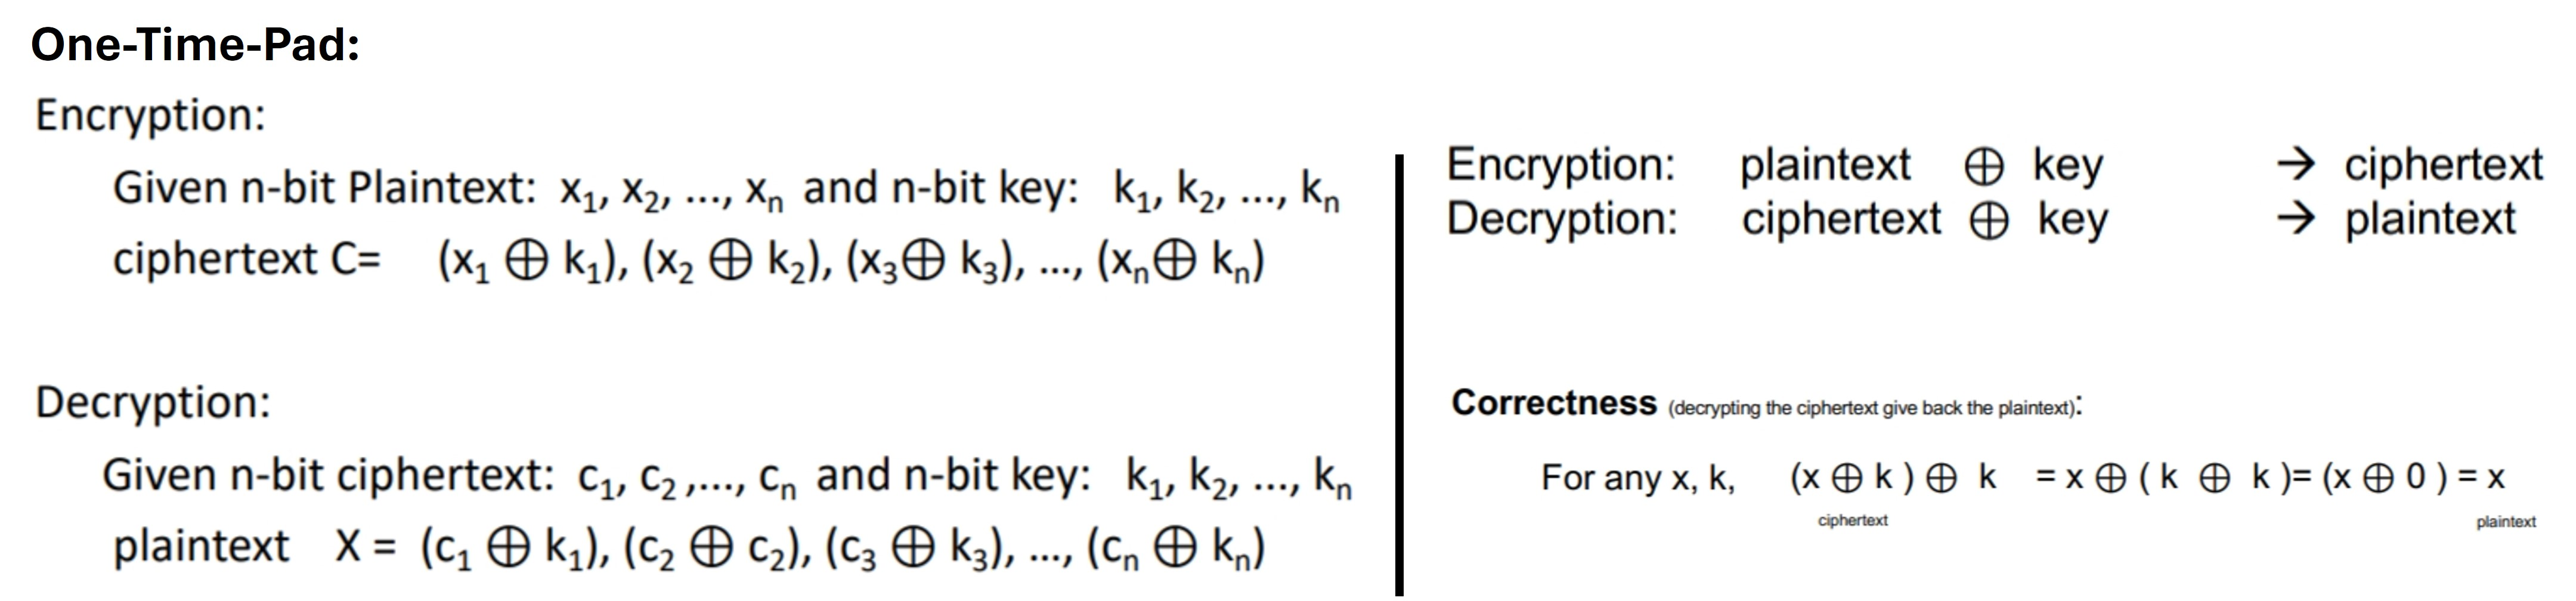
\includegraphics[width=1\linewidth]{OTP}}
\begin{itemize}
\item \textbf{Requirement}: Key cannot be re-used, used only once. Hence, 1GB plaintext would need 1GB key to encrypt.
\item From pair of ciphertext \& plaintext, key can be derived. However, key useless, as only used once.
\item \textbf{Security}: OTP leaks no information of plaintext, sometimes called "unbreakable". There is a exhaustive key for any English sentence. (Perfect Secrecy)
\end{itemize}

\section{Modern Ciphers (Symmetric)}
Generally refers to schemes that use computer to encrypt / decrypt. E.g:
\\ - DES [Data Encryption Standard 1977] 
\\ - RC4 [Rivest's Cipher 4 1987]
\\ - A5/1 [used in GSM 1987]: Used in WEP Wifi 1999, switched to WPA2
\\ - AES [Adv. Encrypt. Std.], RSA).
\begin{itemize}
\item Designs take into consideration of known-plaintext-attack, freq. analysis and other known attacks.
\item Supposed to be secure, so any successful attack does not perform noticeably better than exhaustive search.
\end{itemize}

\subsection{Key Length, Exhaustive Search DES, AES}
\begin{itemize}
\item \textbf{Security of Encryption Scheme}: Quantified by \textbf{length of key}, w.r.t. exhaustive search.
\item Given a key length of 32 bits, there are $2^{32}$ possible keys. Hence, exhaustive search needs to ``loop'' $2^{32}$ in worst case. 
\item \textbf{No. of bits to be considered ``secure''}: 128, 192, 256 bits, \\
- (NIST recommendation for AES).
\end{itemize}

\subsection{1. DES, AES and Exhaustive Search}
\begin{itemize}
\item \textbf{Exhaustive Search on DES}: Key length of DES is 56 bits. Previously, seemed infeasible, but has since become easily broken.
\item \textbf{AES}: New standard for block cipher in 2000, AES block length is 127, key length can be 128, 192 or 256 bits. 
\item Currently, no known attacks on AES. NSA classifies AES as ``Suite B Cryptography''.
\end{itemize}

\subsection{2. Block Cipher \& Mode-of-Operations}
\begin{itemize}
\item \textbf{Block Cipher}: DES \& AES known as ``Block Cipher''. Block cipher designed for some fixed size input/output. \\
- E.g. AES designed for 128 bits input/output.
\item \textbf{Block Cipher Mode Of Operation}: Describes how to repeatedly apply cipher's single block operation to securely transform amounts of data larger than a block. (Extending encryptino from single block to multiple blocks).
\end{itemize}
\centerline{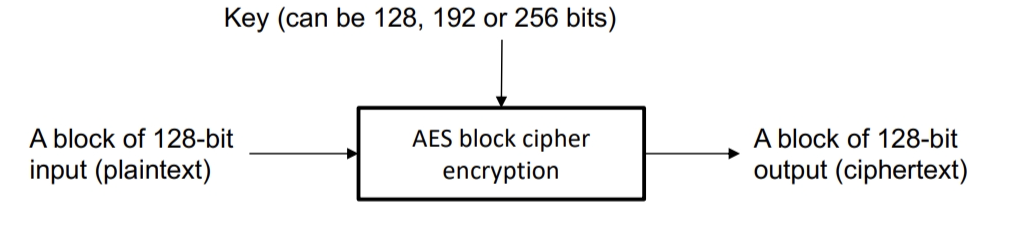
\includegraphics[width=0.8\linewidth]{AES}}

\subsubsection{Mode-of-Operation: ECB Mode on AES}
\begin{itemize}
\item \textbf{Electronic Book Code}: Divide plaintext into blocks, apply block cipher to each block, with the same key.
\item ECB leaks information! AES encryption deterministic without randomly chosen IV.
\item \textbf{Deterministic}: Produces same ciphertext for given plaintext and key over separate executions.
\end{itemize}
\centerline{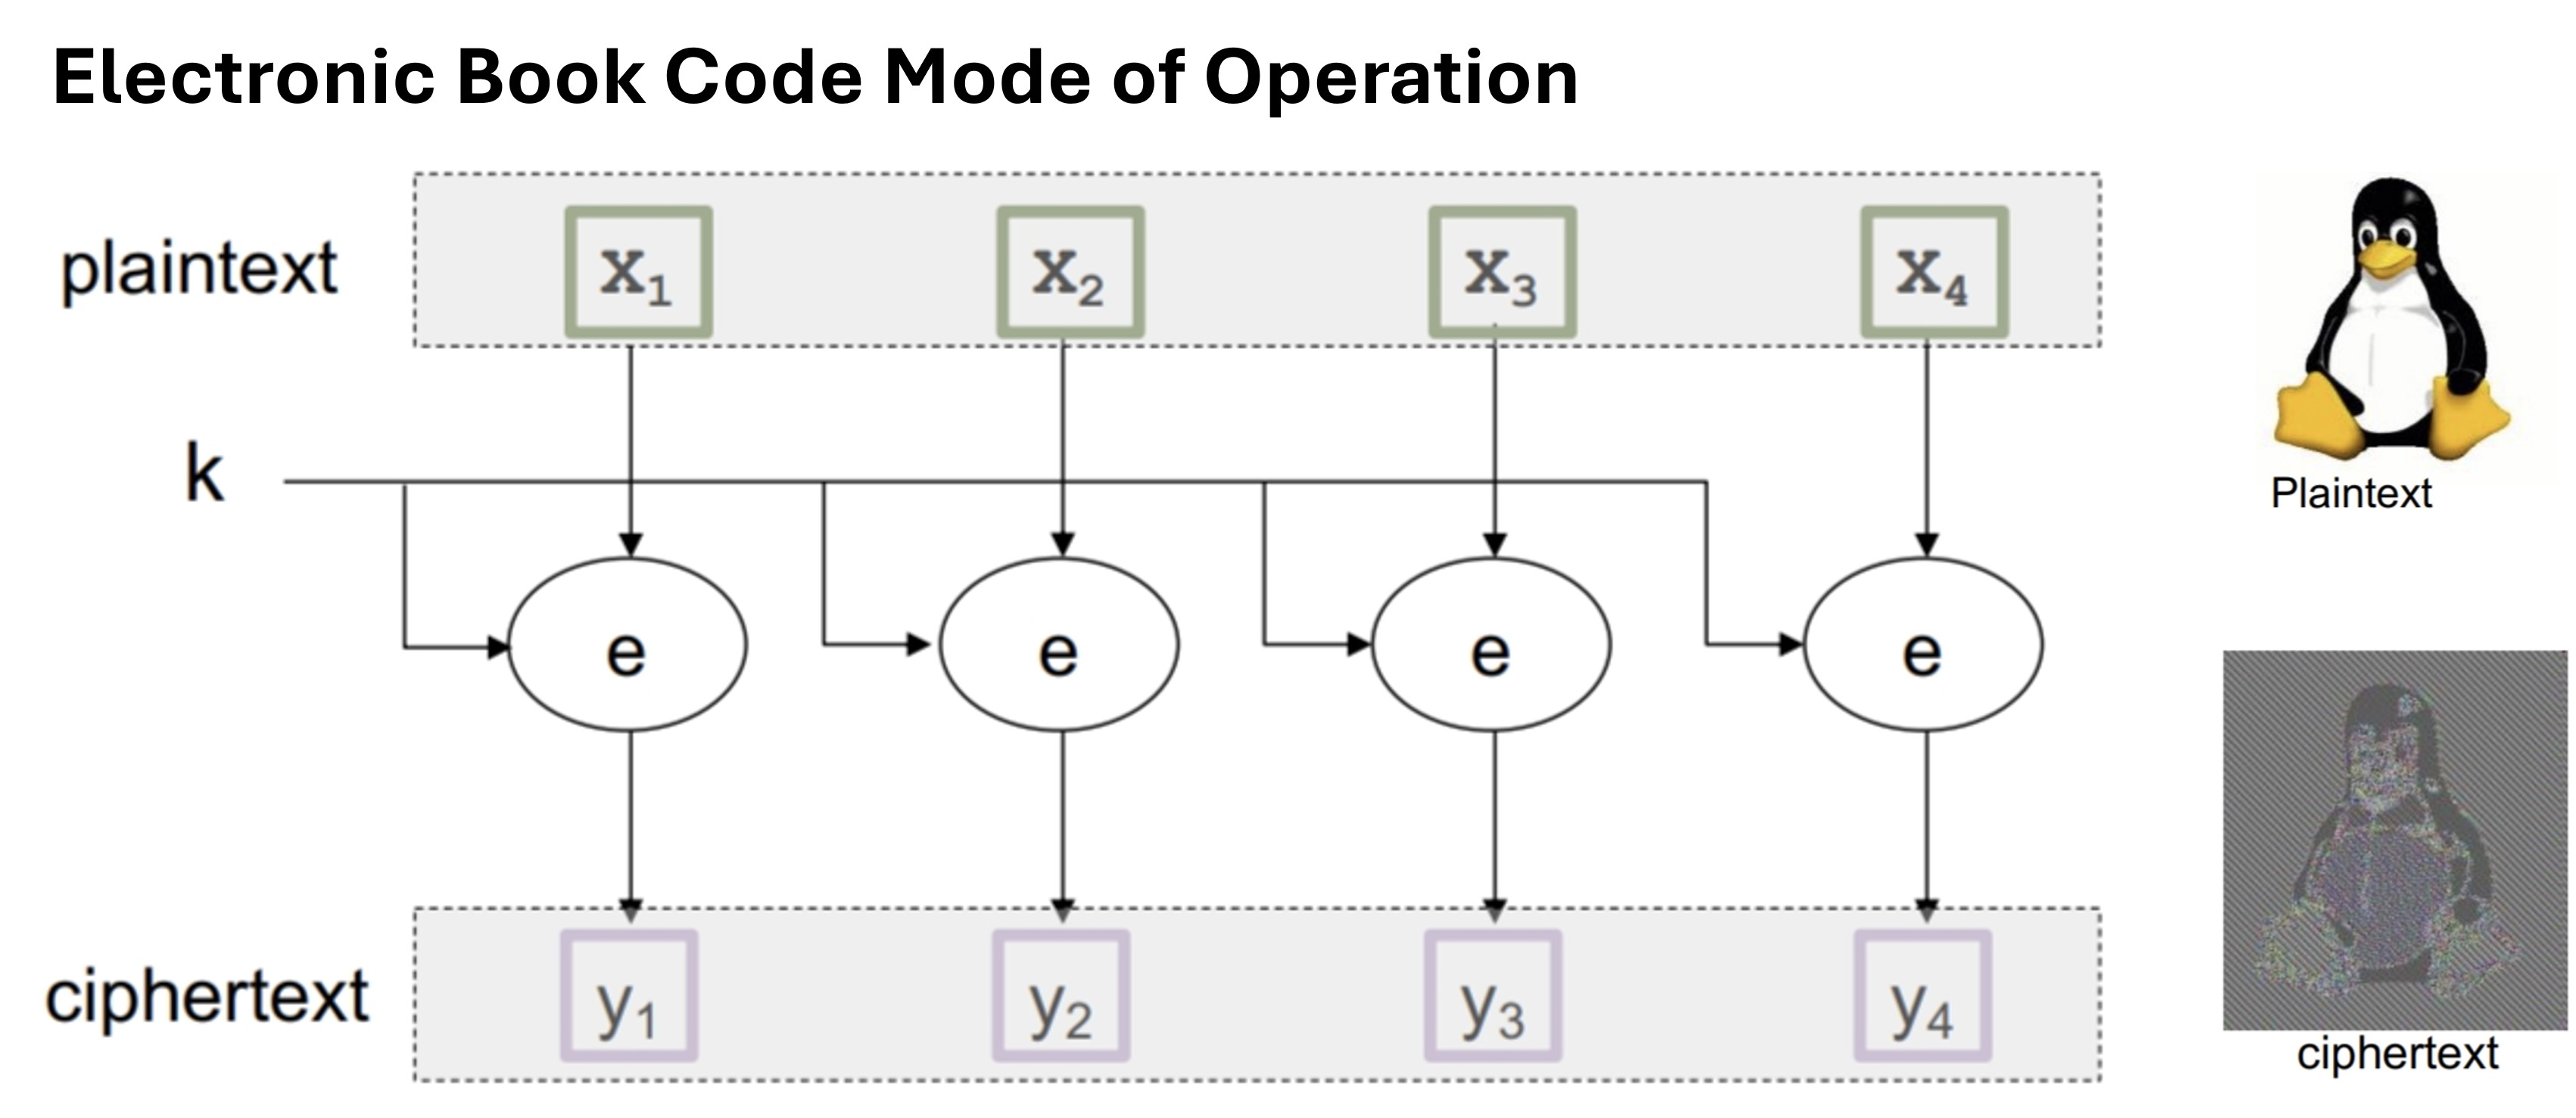
\includegraphics[width=0.7\linewidth]{ECB}}

\subsubsection{Mode-of-Operation: CBC Mode on AES}
\begin{itemize}
\item \textbf{Cipher Block Chaining on AES}: Using an IV, uses chaining process that causes decryption of block of ciphertext to depend on all preceding ciphertext blocks.
\item \textbf{Initialization Vector (IV)}: Arbitrary number of certain length used with secret key, to provide the initial state, for data encryption.
\item \textbf{Encryption}: Each plaintext block is XOR-ed with previous ciphertext block, and then encrypted. Process repeats until all plaintext is ciphertext blocks.
\item \textbf{Decryption}: Reverse encryption process. Note, process does not need to start with final block, can happen simultaneously as all inputs present.
\end{itemize}
\centerline{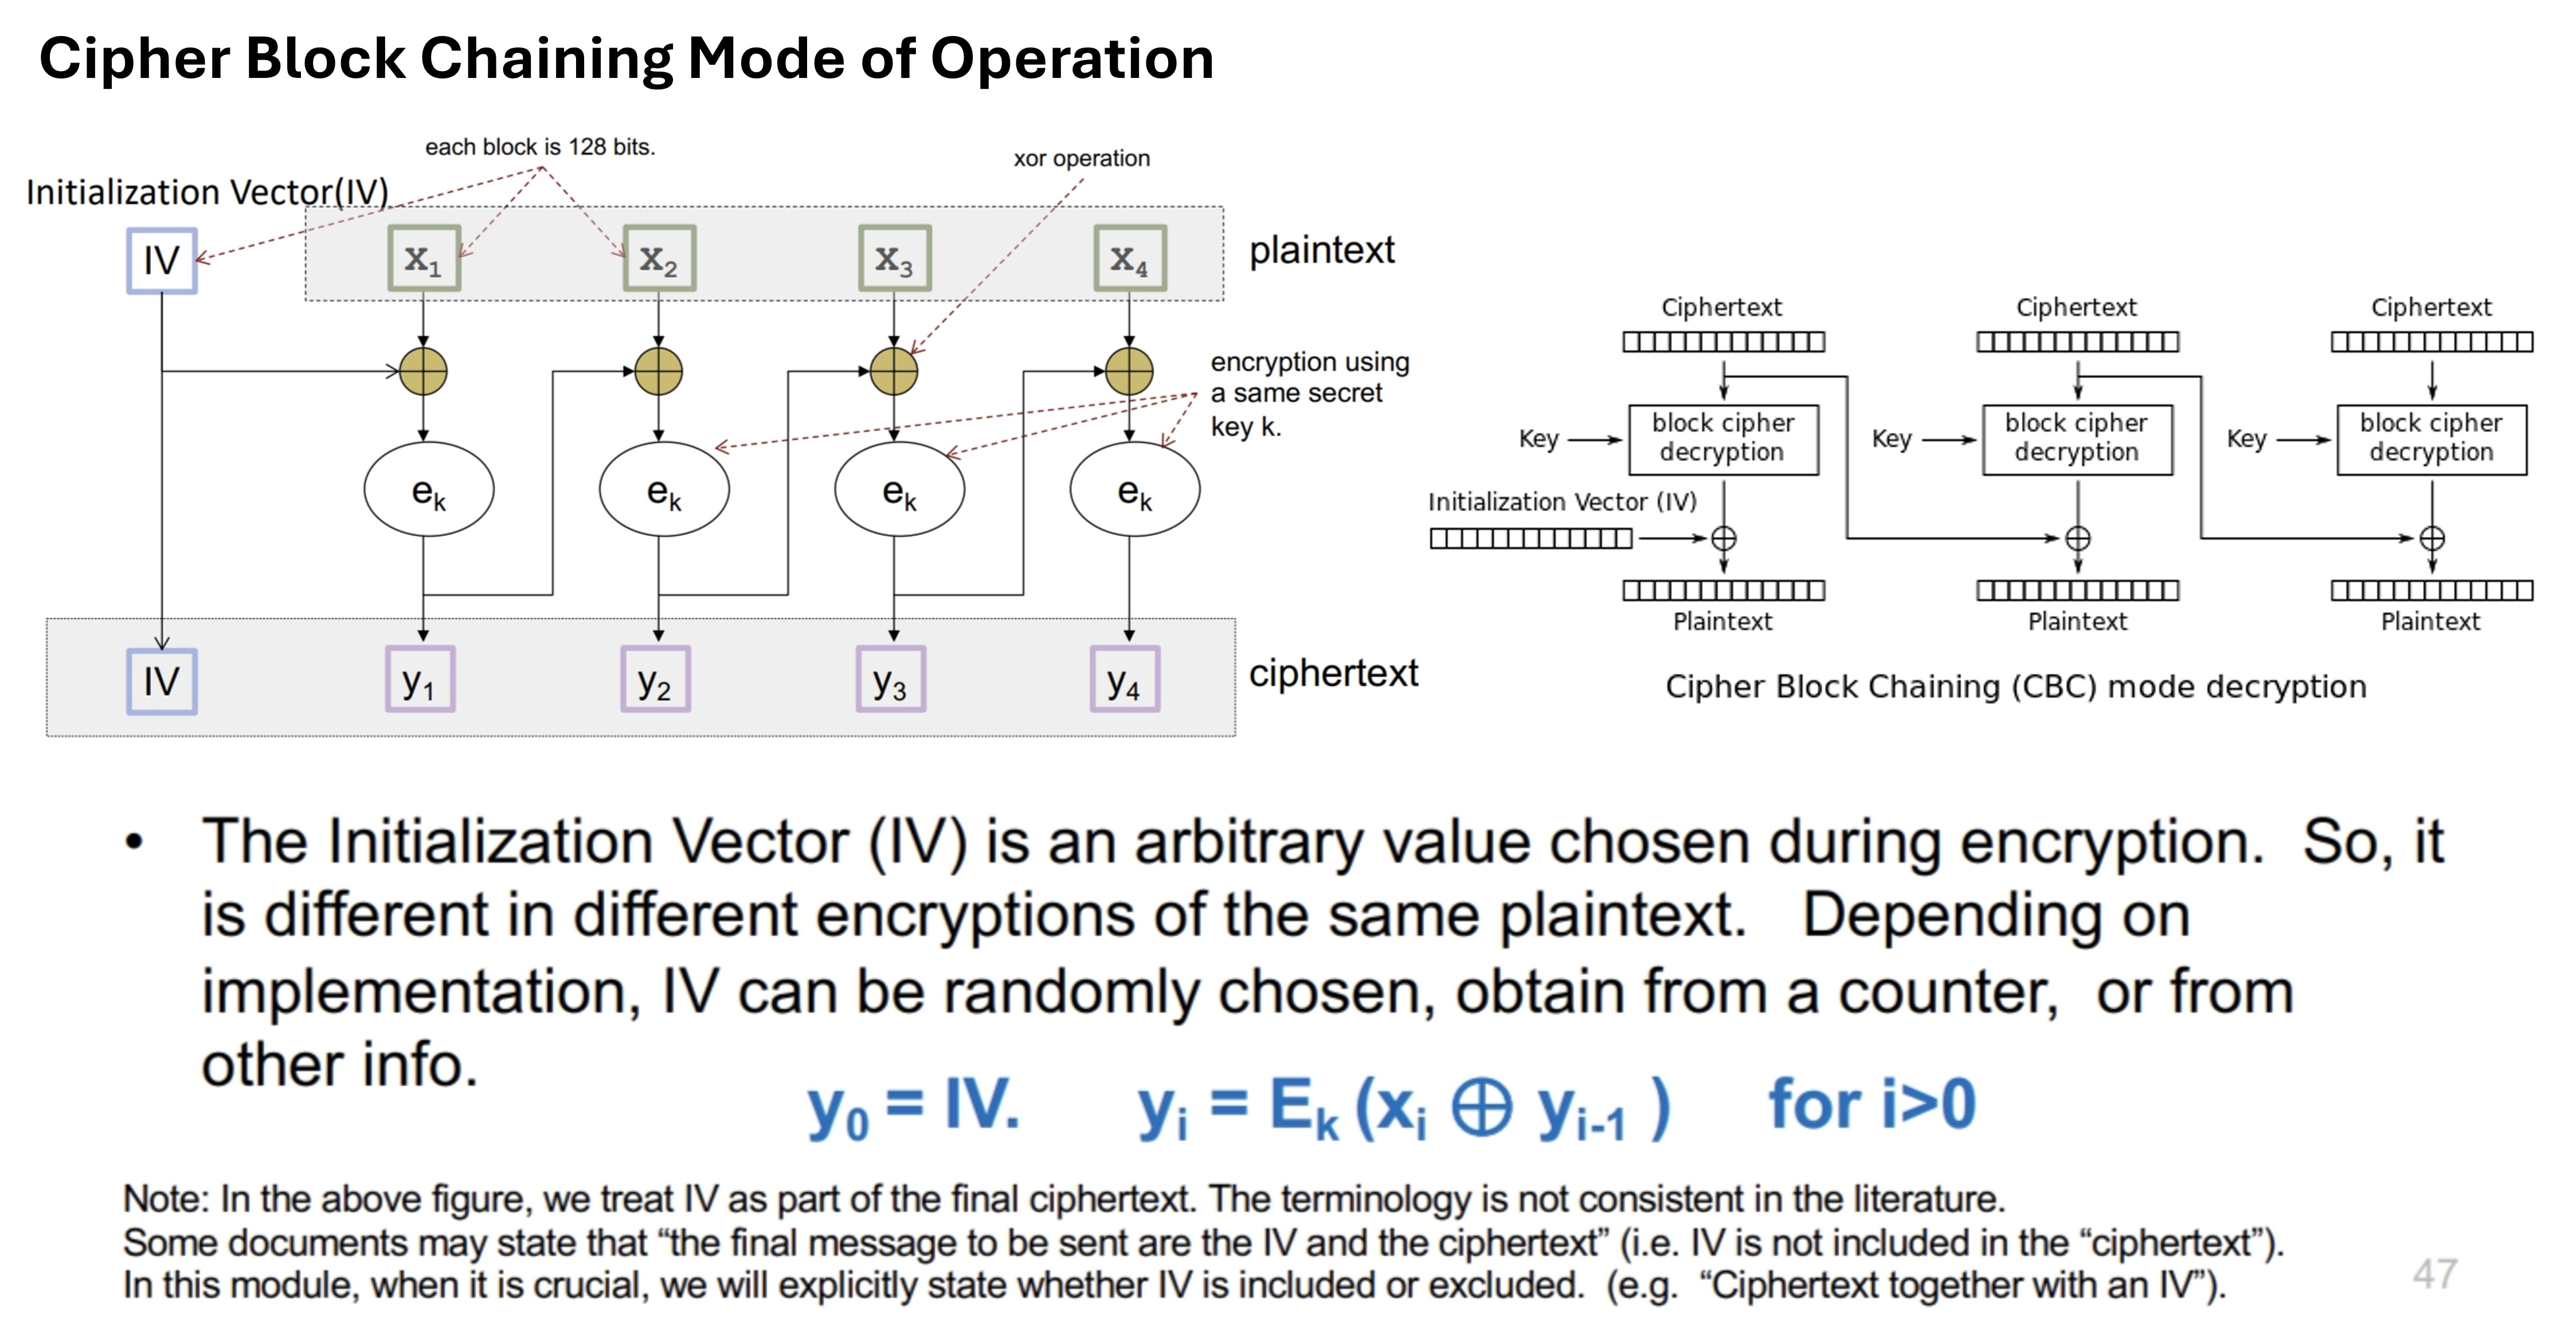
\includegraphics[width=1\linewidth]{CBC}}

\columnbreak
\subsubsection{Mode-of-Operation: Counter Mode (CTR) on AES}
\begin{itemize}
\item \textbf{Counter Mode}: Turns block cipher into stream cipher, generates next keystream block by encrypting successive values of a ``counter''. Counter can be any function producing sequence, incld. simple increment by one counter.
\end{itemize}
\centerline{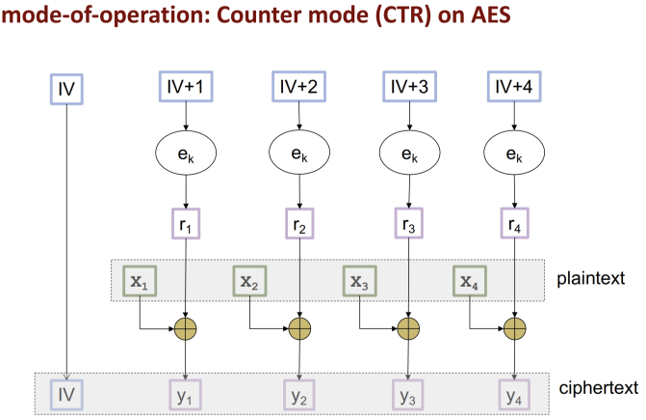
\includegraphics[width=0.5\linewidth]{CTR}}

\subsubsection{Mode-of-Operation: GCM Mode (Galois/Counter)}
\begin{itemize}
\item \textbf{GCM}: Combines Counter mode (CTR) with Galois authentication. Construction of mode more complicated, is ``Authenticated-Encryption''.
\item Ciphertext consists of extra tag for authentication, secure in presence of decryption oracle.
\end{itemize}

\subsubsection{Python Programming: CBC}
\centerline{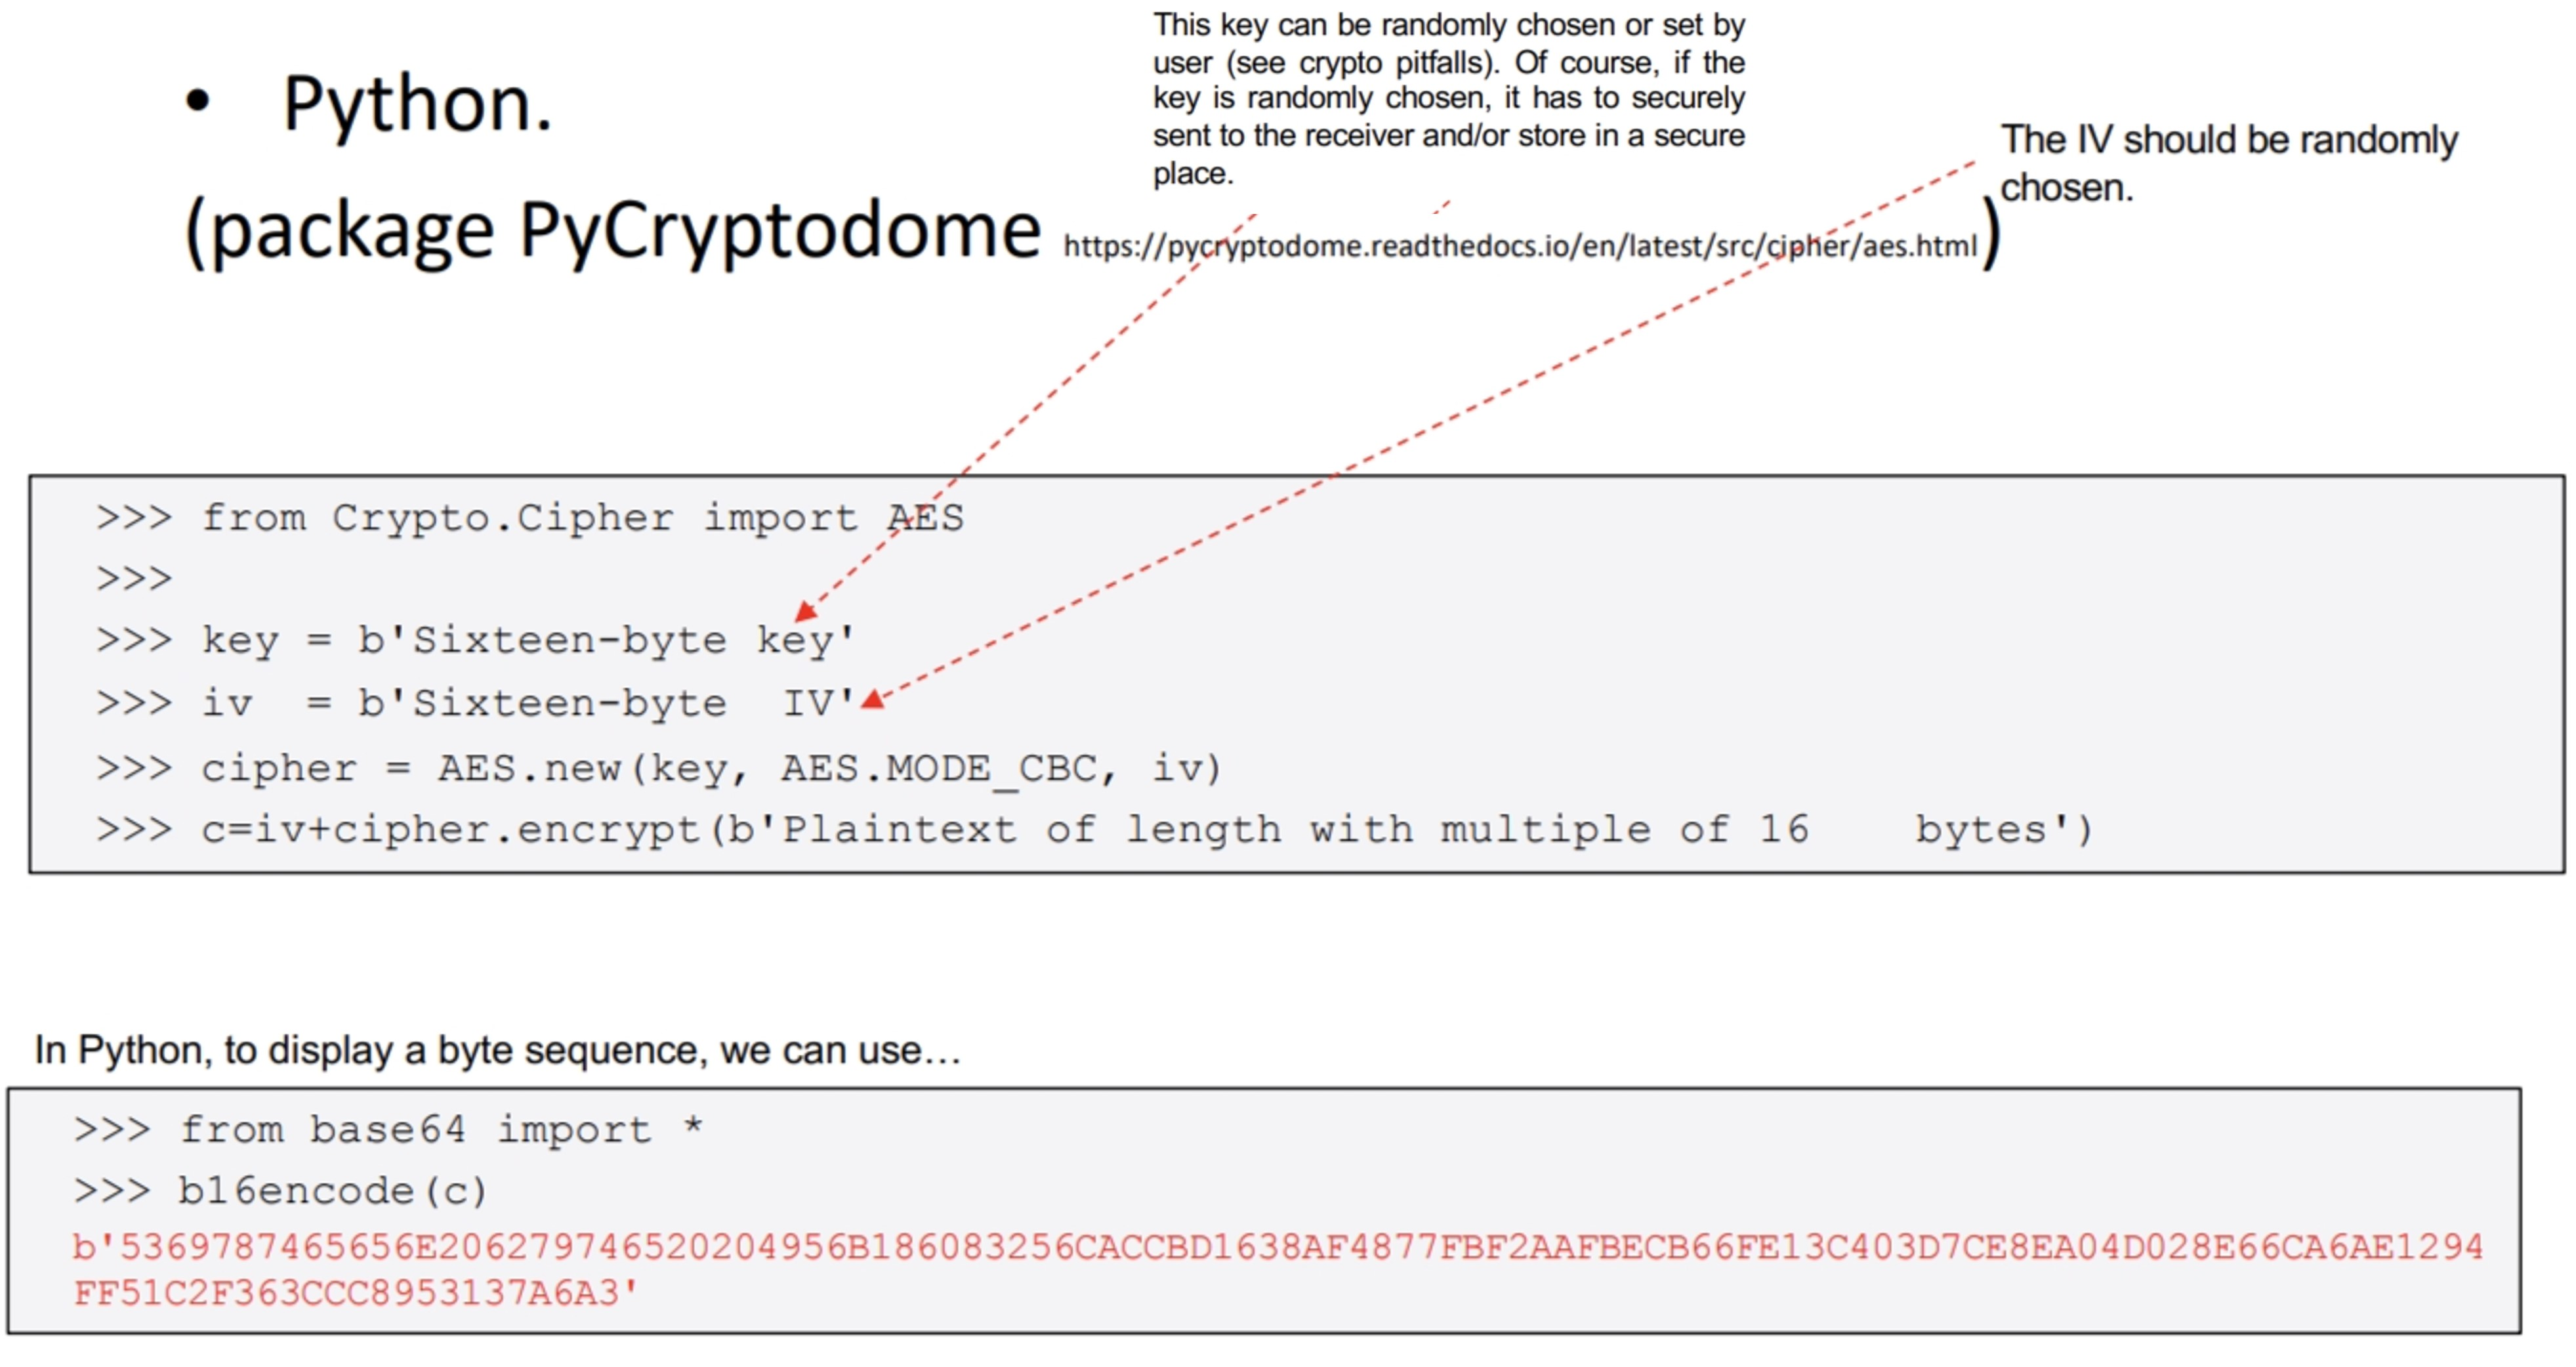
\includegraphics[width=0.95\linewidth]{CBCProgramming}}

\subsection{3. Stream Cipher and IVs}
\subsubsection{Stream Cipher}
\begin{itemize}
\item \textbf{Stream Cipher}: A symmetric key cipher where plaintext combined with \textbf{pseudorandom cipher digit stream (keystream)}.
\item ``Inspired'' by one-time-pad, generate some cryptographically secure pseudorandom sequence. 
\item w/o knowing secret key, computationally diff. to distingush from truly random sequence. Similarly diff. to get short secret key from sequence, or predict part of sequence from another part.
\item \textbf{IV}: Most ciphers have \textbf{Initialization Vector}, randomly chosen or from counter.
\end{itemize}
\centerline{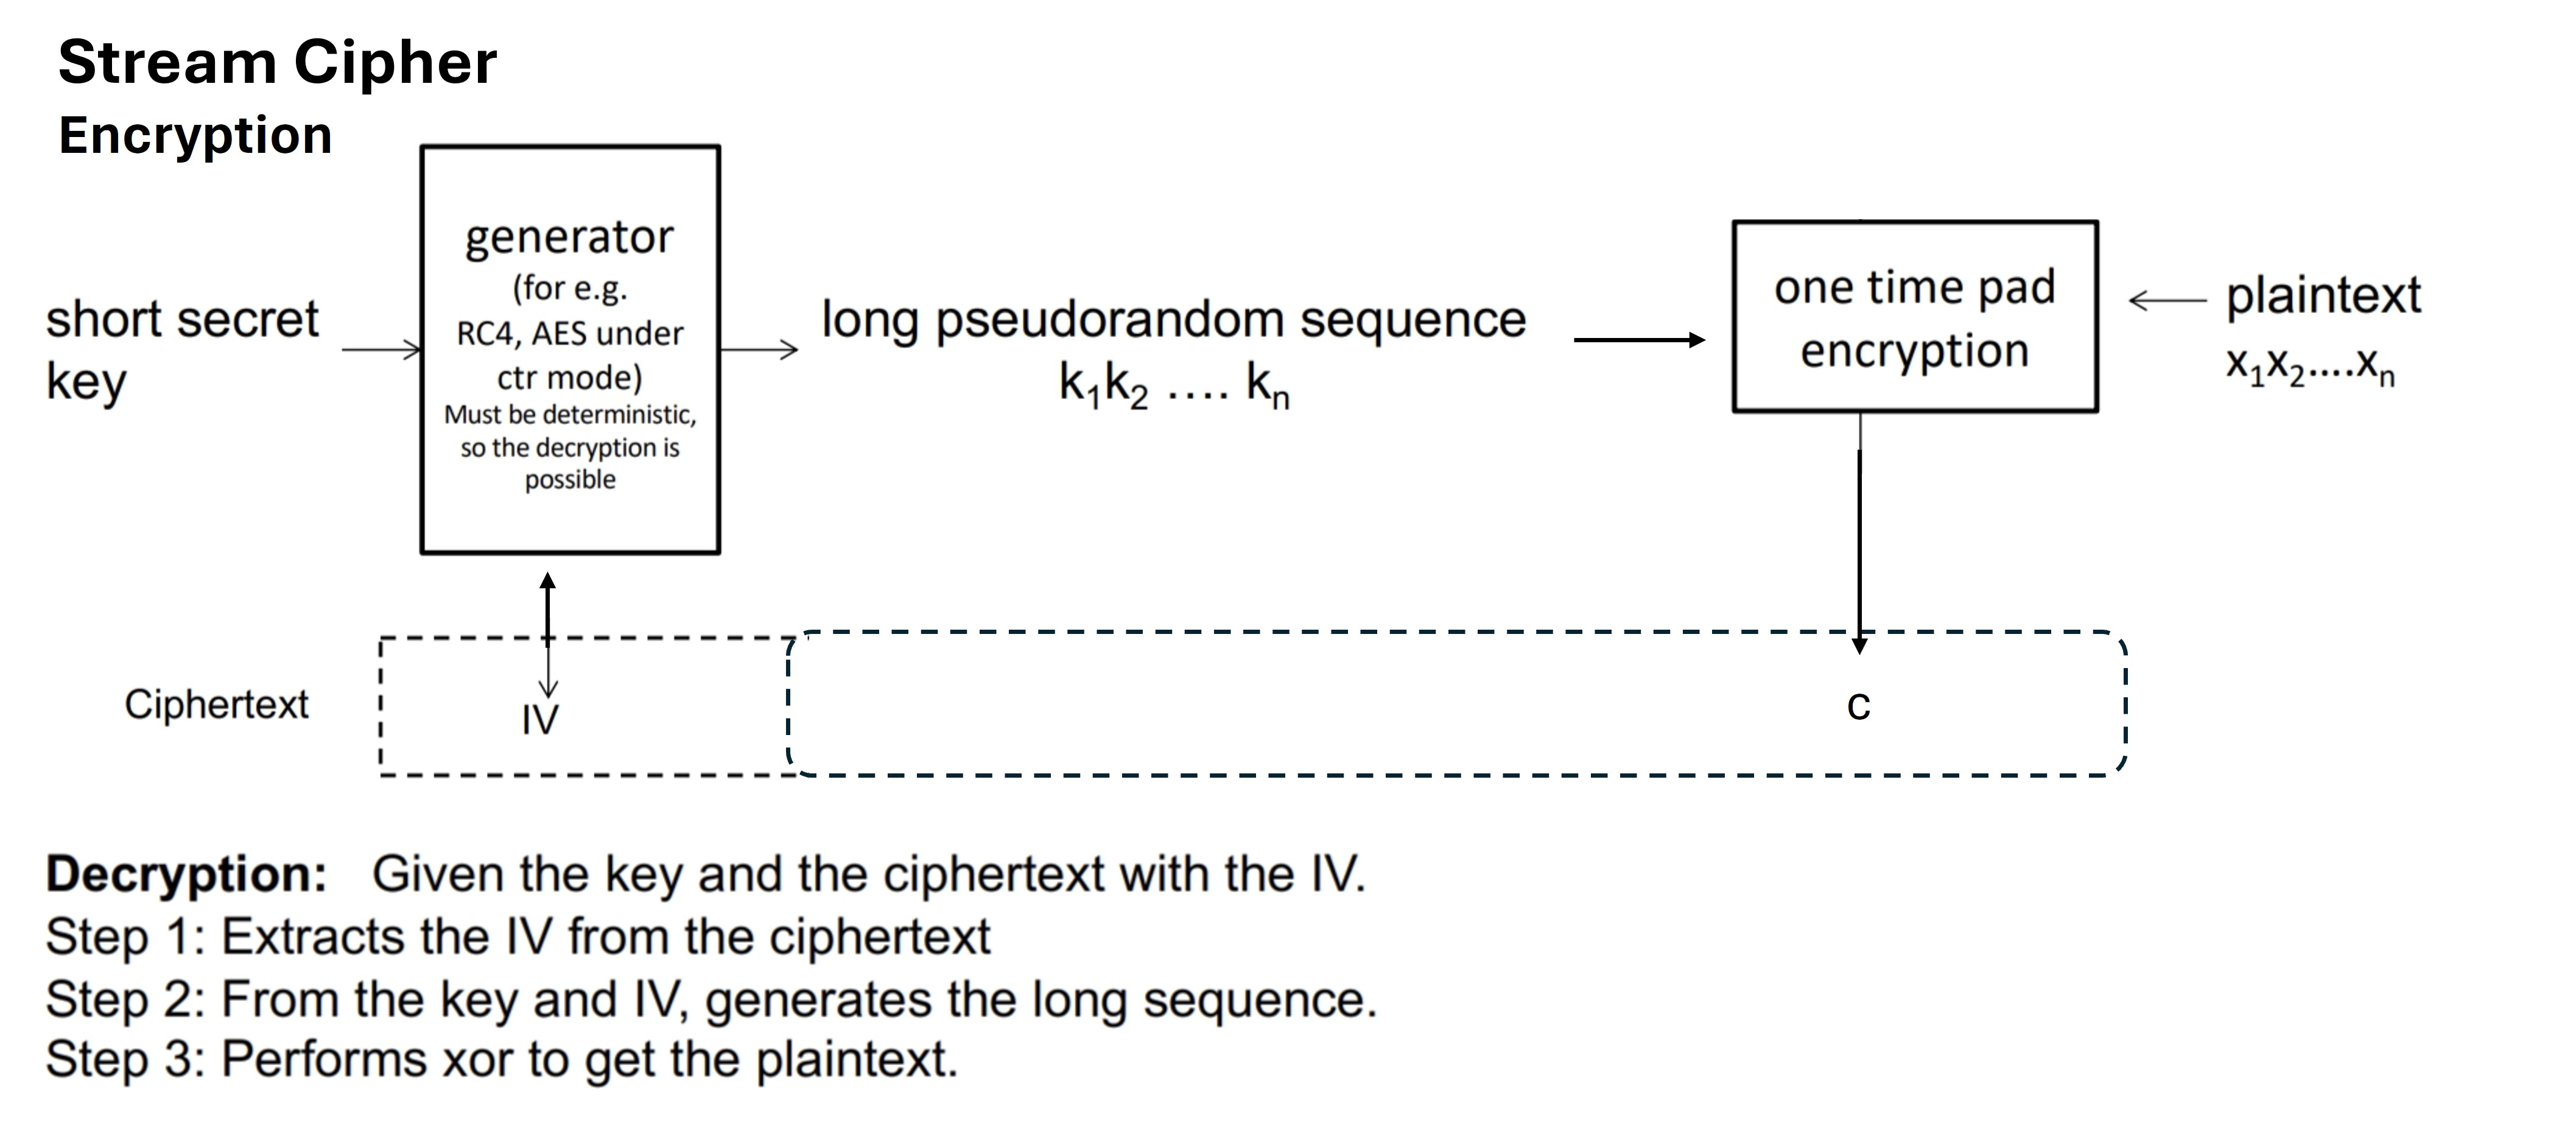
\includegraphics[width=0.95\linewidth]{streamCipher}}

\subsection{Role of Unique IV}
\begin{itemize}
\item Recall, IV appended to front of $c$ to form ciphertext. This IV must be different for every message. IV need not be secret.
\item Sequence is derived from IV and secret key. IV needs to be unique for every message! Otherwise, leaks information.
\item \textbf{Unique IV}: If IV different, two pseudorandom sequences will be different. Two ciphertexts of same plaintext will be different. Can just randomly choose the IV for each message.
\item Hence, xor'ing two ciphertexts will not cancel out pseudomsequences.
\item \textbf{IV makes encryption ``probabilistic.}
\end{itemize}
\centerline{\includegraphics[width=0.95\linewidth]{uniqueIV}}
\begin{itemize}
\item IV also needed in \textbf{CBC mode}, to make encryption non-deterministic. If encryption deterministic (without IV), it will leak information on whether plaintext of two ciphertext are the same, if $C_1 == C_2$. Could be crucial piece of information.
\end{itemize}


\section{Types of Attacks}

\subsection{Meet-In-The-Middle Attack (Double / Triple DES)}
\subsubsection{Double / Triple DES}
\begin{itemize}
\item \textbf{Double / Triple DES}: To improve DES security, (DES weak as key length of 56 bits short), do multiple repeated encryption using different keys. A reason for this may be to utilize already existing suitable hardware to encrypt.
\item DES does not form a group ( $E_{k1} ( E_{k2} (x) ) \neq E_{k2} (x) $) for some $k3$, so makes sense to use multiple encryption.
\item \textbf{Double DES}: Consider double encryption, we expect key-strength to be 112. ($2^{56 + 56}$). However, attacker, with storage space, can reduce key strength to below 57.
\end{itemize}

\subsubsection{Meet-In-The-Middle Attack}
\begin{itemize}
\item \textbf{MITM}: Meet-in-the-middle Attack, a well-known plaintext attack, is a generic space-time tradeoff cryptographic attack against encryption schemes that perform multiple encryption operations in sequence.
\item Breaking two-part encryption from both sides simultaneously.
\item Primary reason why \textbf{Double DES not used}, and why \textbf{Triple DES key} (168-bit) can be brute forced by attacker with $2^{56}$ space and $2^{122}$ operations.
\item \textbf{Mechanism}: Assume attack has a \textbf{pair ($m, c$)} of plaintext and corresponding ciphertext.
\item \textbf{Remedy}: Use triple encryption, but with 2 keys. (E.g. 3DES, TDES, 3TDES etc.)
\end{itemize}
\centerline{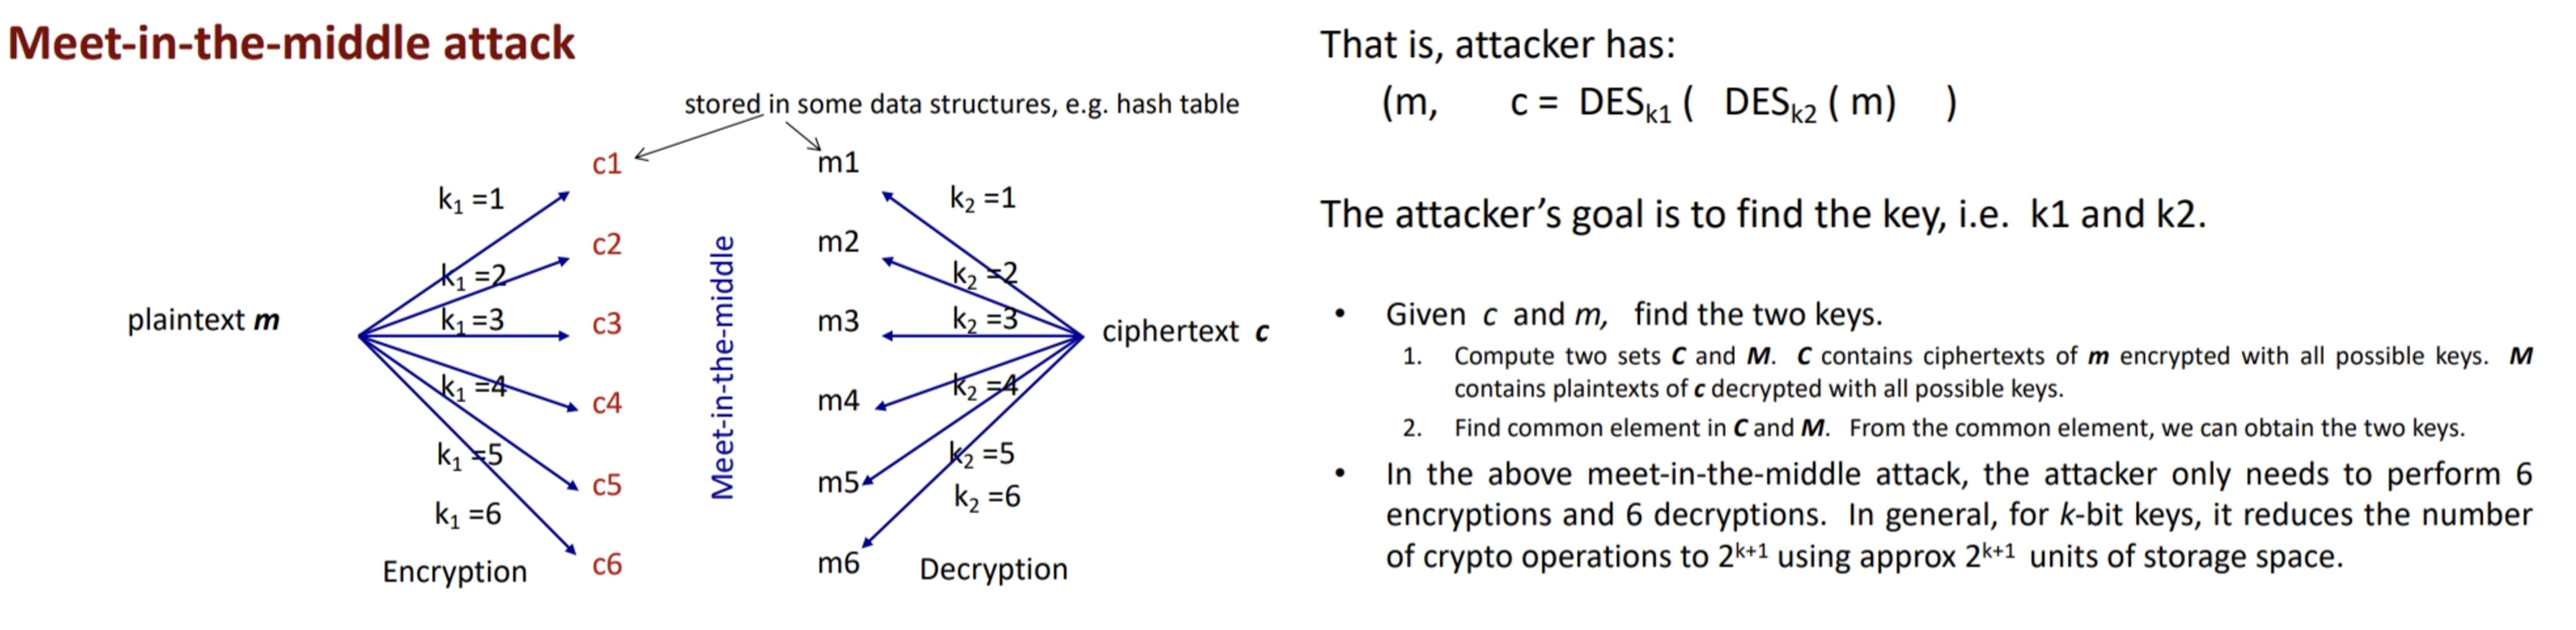
\includegraphics[width=1\linewidth]{MITM}}


\subsection{Padding Oracle Attack}
\subsubsection{Padding Format}
\begin{itemize}
\item For fixed size blocks, e.g. block size of AES is 128bits (16 bytes), padding is needed to fit plaintext into last block.
\item Many ways to fill value, but important piece of information encoded: \textbf{number of padded bits}. If information missing, receiver will not know lenght of plaintext.
\item E.g. \textbf{PKCS\#7 Padding Standard.}
\end{itemize}
\centerline{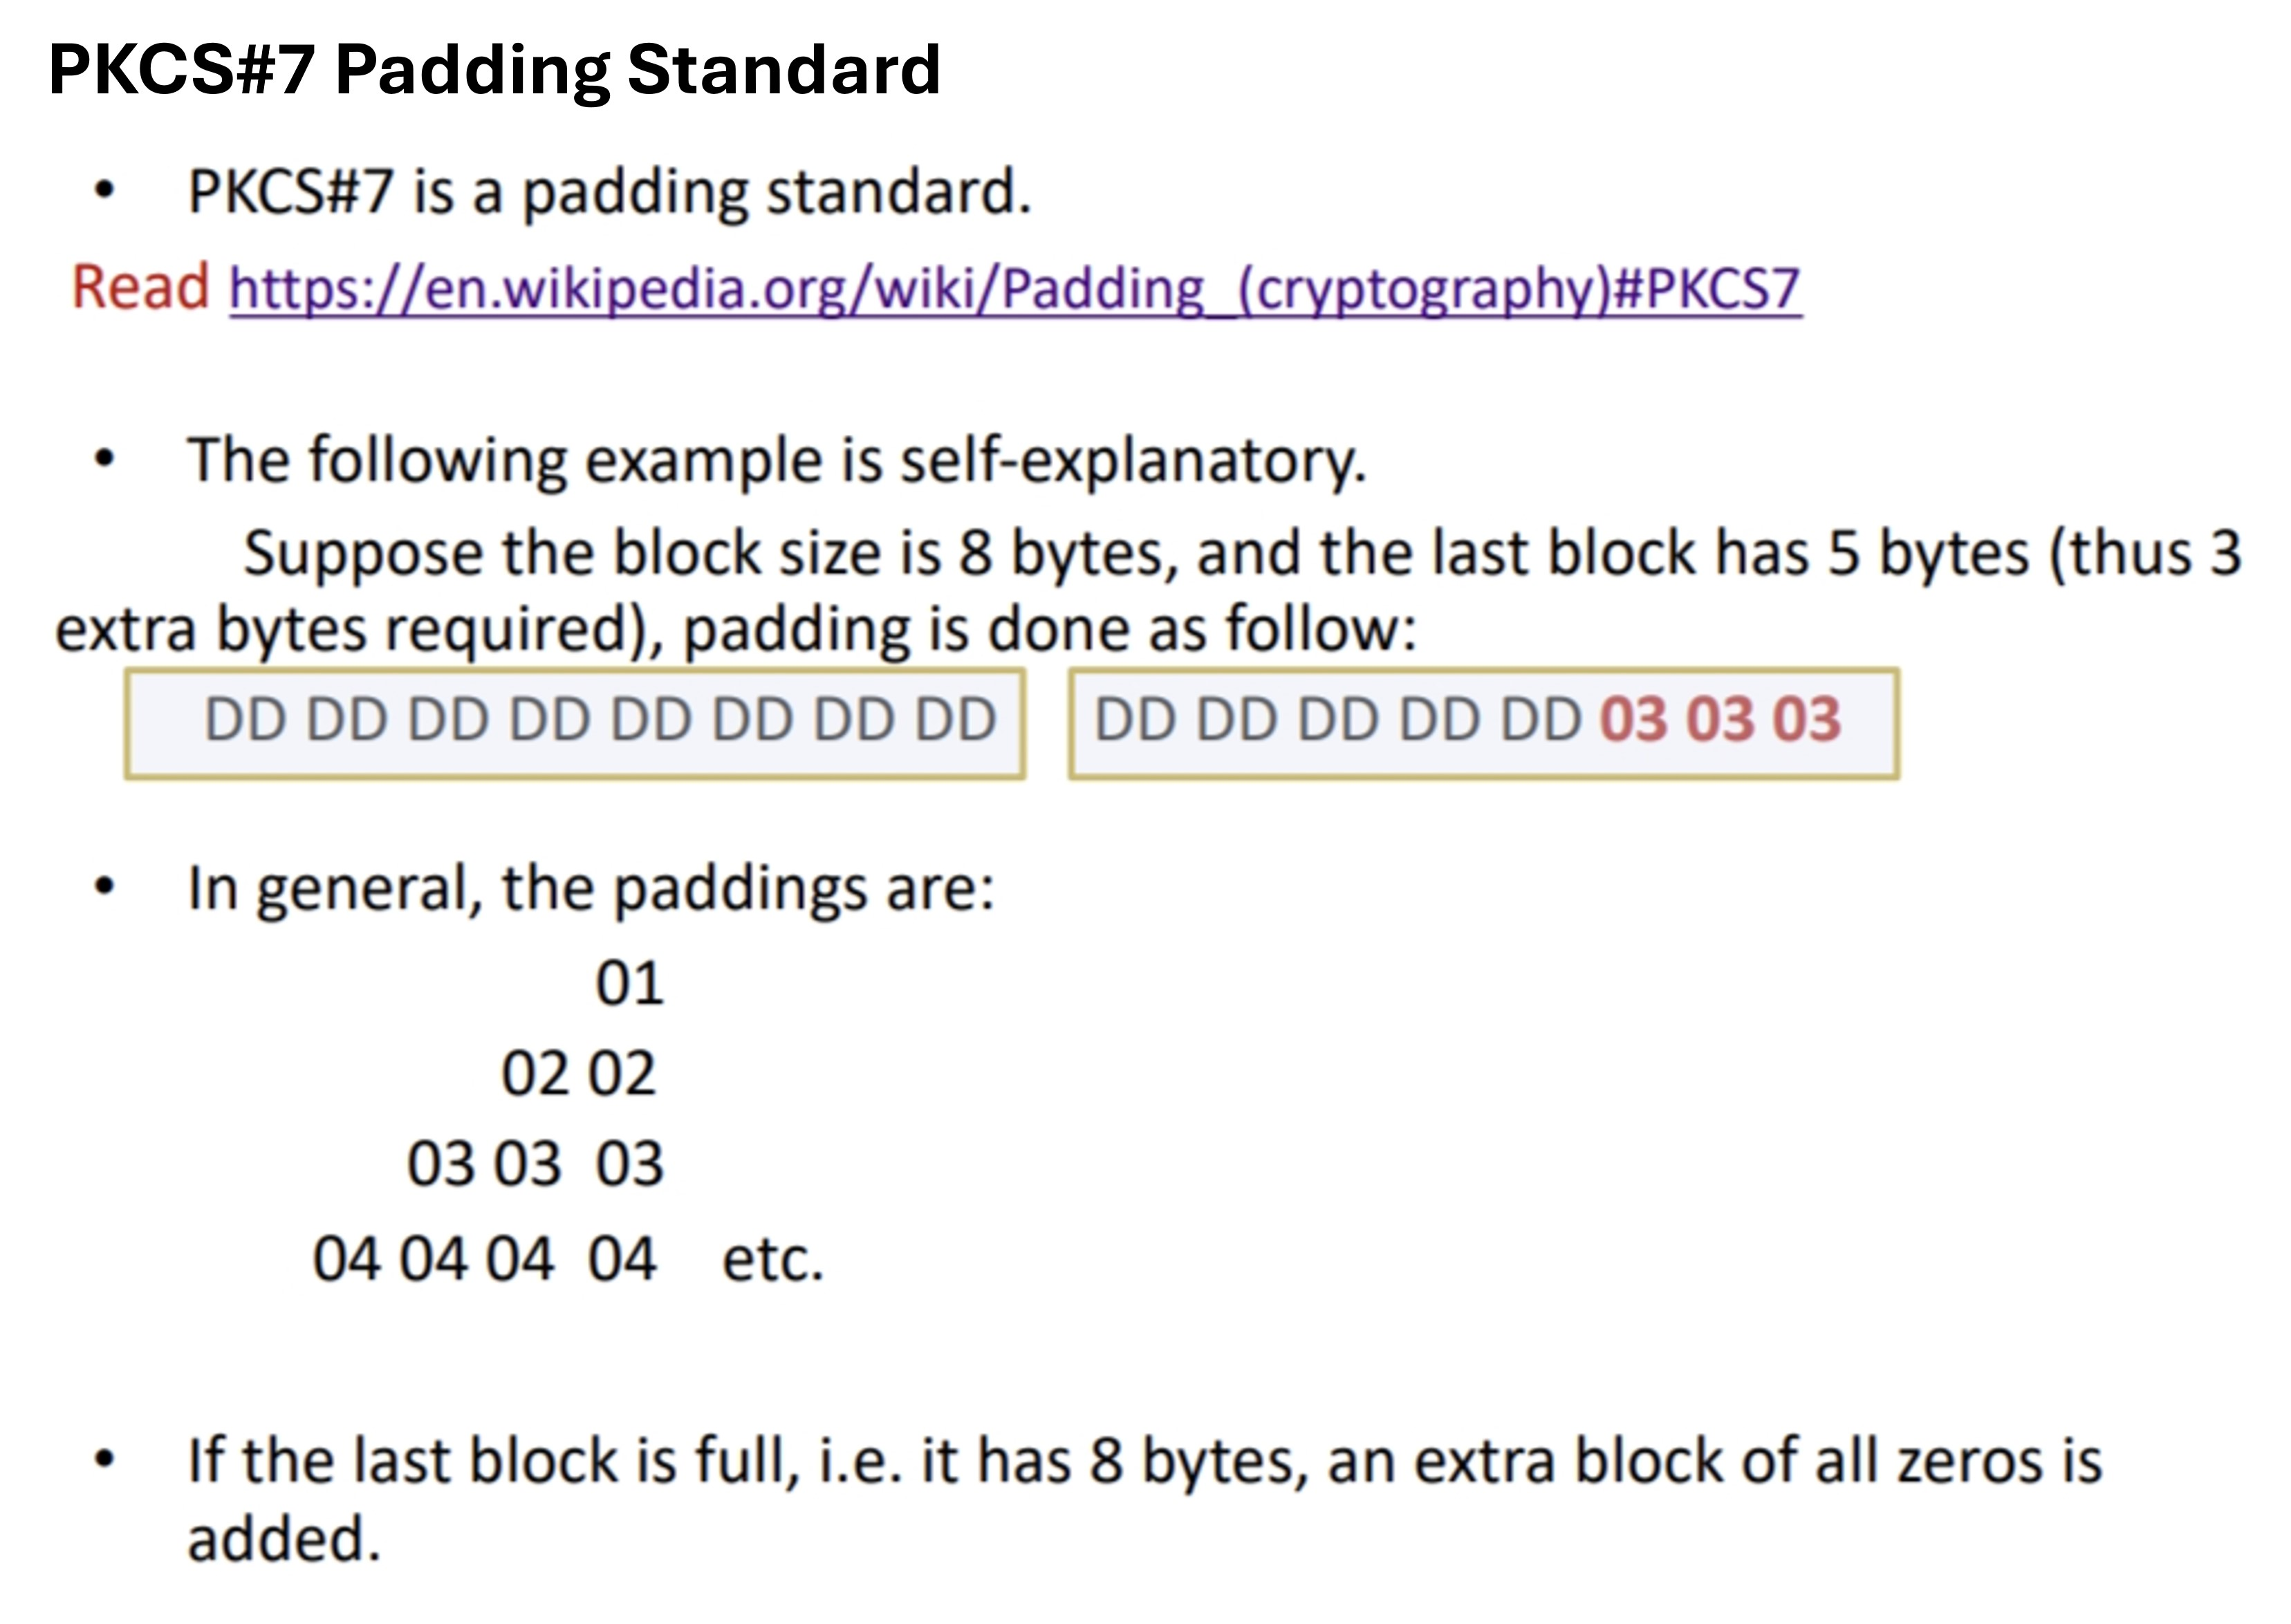
\includegraphics[width=0.8\linewidth]{PKCS7}}

\subsubsection{Oracle}
\begin{itemize}
\item \textbf{Security Analysis}: Need to know \textbf{1. information attackers have}, 2. attacker's goals.
\item \textbf{Oracle}: Query-answer system. Attacker can send in multiple queries, \textbf{Oracle} will output the answer. E.g. \\
-  \textbf{Encryption Oracle}: Output ciphertext for given plaintext, of s. key $k$. \\
-  \textbf{Decryption Oracle:} Output plaintext given ciphertext, of s. key $k$.
\item \textbf{Padding Oracle}: Attacker can query a ciphertext (encrypted using some secret key $k$, padding oracle knows $k$). Oracle outputs yes/no if plaintext is in correct ``padding'' format.
\item Padding Oracle can come in many forms, e.g. query response behavior, response time, subtle differences.
\item \textbf{Padding Oracle Attack Model}: \\
- Attacker has ciphertext including iv: (iv, $c$) \\
- Attack's goal: plaintext of (iv, $c$).
\end{itemize}

\subsubsection{Padding Oracle Attack (on AES CBC Mode)}
\begin{itemize}
\item AES CBC mode not secure against padding oracle attack. (In particular, when done with PKCS\#7).
\item Easily extend algorithm to find all plaintext. Attack is practical as there are protocols between client and server which performs this. \textit{Now, if attack obtained ciphertext, attack can interact with server to get plaintext.}
\item \textbf{Prevention of Padding Oracle Attack}:
	\begin{itemize}
	\item Deny access to such Oracle. Might not be feasible all the time.
	\item Change padding standard to mitigate attack. However, may be smarter way to attack new padding.
	\item Using CTR mode might avoid padding. In practice, bit strings have to be padded in one way or another.
	\item Padding Oracle weaker form of Decryption oracle. If scheme secure in presence of decryption oracle, scheme also secure against padding oracle attack. GCM believed to be IND-CCA2 secure.
	\end{itemize}
\end{itemize}

\columnbreak
\subsubsection{Padding Oracle Attack Algorithm}
\begin{itemize}
\item \textbf{Algorithm}: \\
- Force last X bytes to be padding \\
- Do this by modifying byte of previous ciphertext/IV (Loop till YES) \\
- Here, by XOR'ing padding and input, we get intermediate byte. \\
- By XOR'ing this int. byte with original IV / ciphertext, find plaintext!
\item \textbf{Easily extend algorithm} to find all plaintext, by using increasing length of padding, decrypt from end to start. (Right to Left, repeat process).
\end{itemize}
\centerline{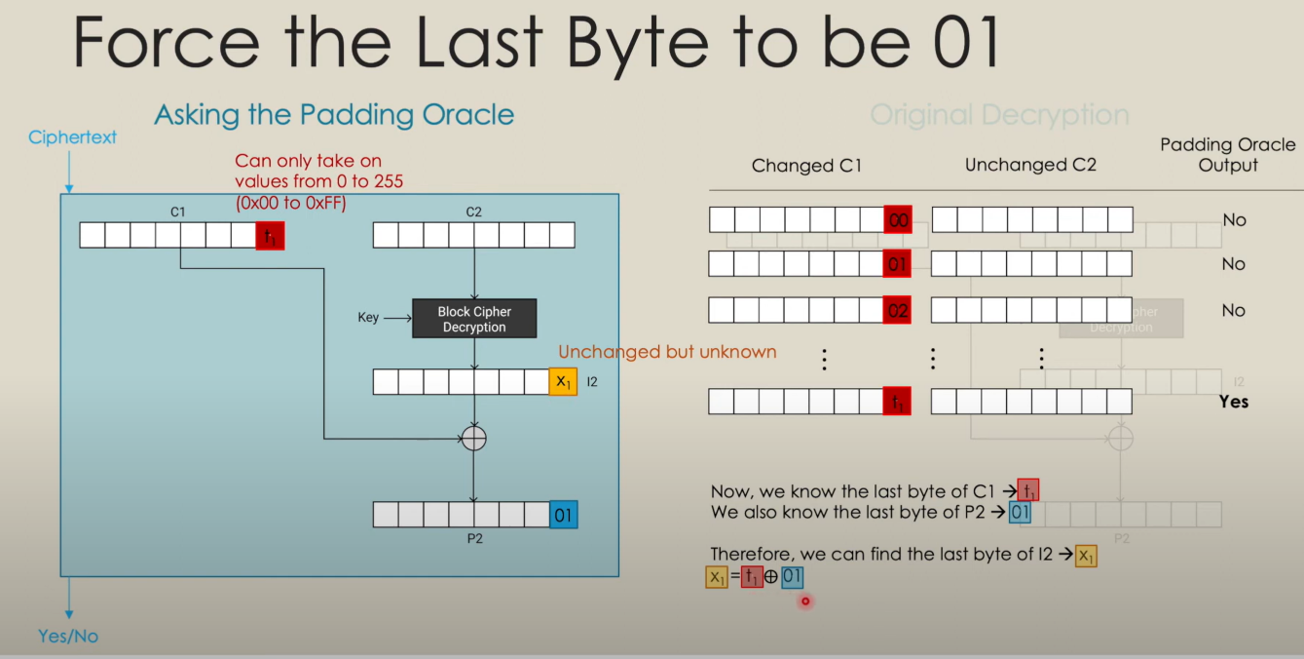
\includegraphics[width=0.8\linewidth]{paddingOracle1}}
\centerline{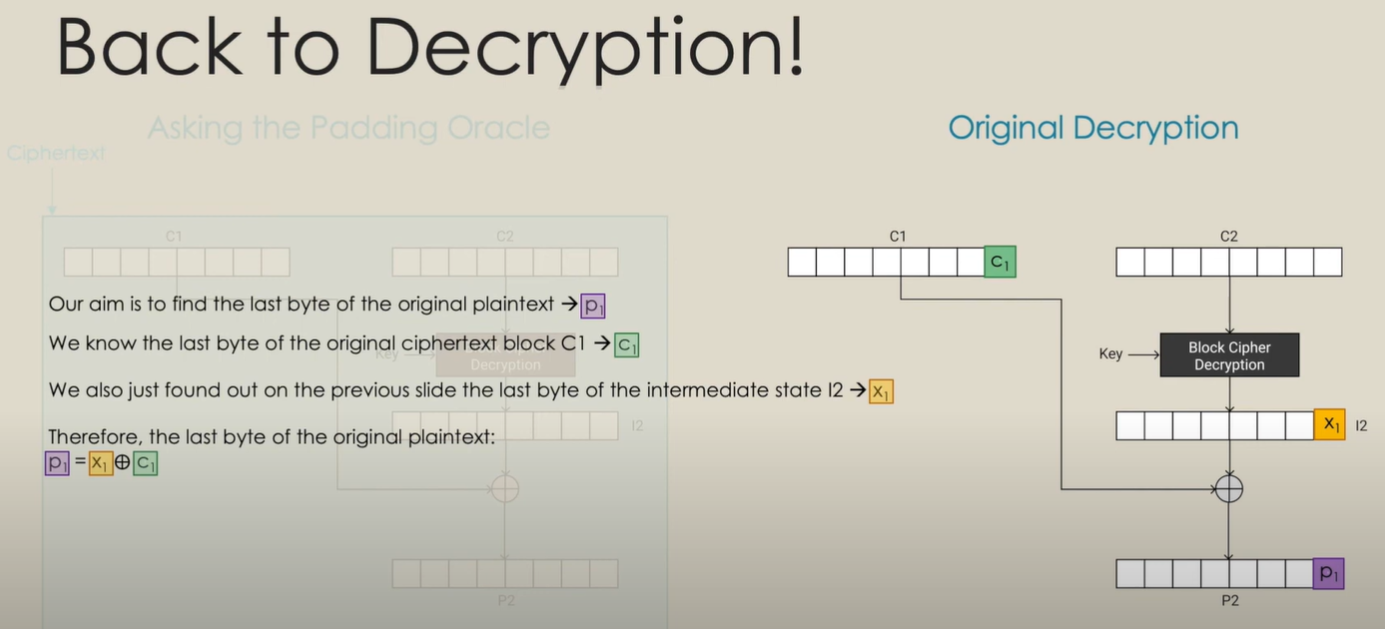
\includegraphics[width=0.8\linewidth]{paddingOracle2}}

\section{Cryptography Pitfalls}
\begin{itemize}
\item Any secure encryption scheme can be vulnerable if not implemented or adopted properly. Examples include: \\
\textbf{- Predictable Randomness}: Secret key generated predictable, compromise security \\
\textbf{- Modify/Design own encryption scheme}: ``Don't roll your own crypto /security protocol''. Use standard library.
\end{itemize}

\subsubsection{Wrong choice of IV}
\begin{itemize}
\item \textbf{IV Generation}: IV's must not be same for two different ciphertext. 
\item E.g. To encrypt file F, IV derived from filename/meta-data. 
\item E.g. \textit{Microsoft RC4 [implementation] Flaw}, in both Word and Excel, where same IV used when document modified, causing part of documents recovered with negligible amount of computation.
\item When using AES under CBC mode, IV should be unpredictable to prevent certain attack. (E.g. IV = 1, 2, 3). BEAST attack exploits this.
\item \textbf{Reusing one-time pad}: E.g. US Verona Project against Soviets.
\end{itemize} 

\subsubsection{Reliance on Obscurity: Kerchoff's Principle}
\begin{itemize}
\item \textbf{Principle}: System should be secure even if everything about system, except secret key, 
is public knowledge.
\item \textbf{Security through Obscurity}: To hide design of system to achieve security. Not advisable to reveal certain settings (network structure, settings, algorithm, implementation, usernames etc). Obscurity as additional layer in defense-in-depth strategy. Deter, discourage novice attackers.
\item E.g. \textbf{Against relying on Obscurity}: RC4 algorithm was trade secret, but was anonymously posted. MIFARE Classic smartcard also reversed-engineered.
\end{itemize}


\section{2. Authentication Credential}
\begin{itemize}
\item \textbf{Authentication Credential} as any data (PIN, digi. certificate, password) or device that is issued to individual / system used to authenticate identity for purposes of facilitating access.
\item \textbf{Authentication}: Process of assuring communicating entity or origin of piece of information is one it claims to be.
\item \textbf{Authenticity implies integrity}.
\end{itemize}
\centerline{\includegraphics[width=1\linewidth]{communicatingEntity}}
\begin{itemize}
\item \textbf{Authentication Process}: 
	\begin{itemize}
	\item For \textbf{data-origin auth}, one way is to use crypto scheme such as Signature, or MAC (message auth. code).
	\item For \textbf{communication entity auth}, need some authentication protocol employing above crypto primitives.
	\end{itemize}
\item \textbf{Credential}: Unforgeable info required for authentication. (E.g. password is an authentication credential.)
\end{itemize}

\subsection{2.1 Password}
\subsubsection{Password System}
\begin{enumerate}
\item \textbf{Bootstrapping}: User, server establish common password, server keeps file recording identity \textit{(userid, username)} \& \textit{password}. \\
- (Bootstrapping, establish user chosen /or default password.)
\item \textbf{Authentication}: Server authenticates entity. Entity who gives correct password to claimed identity authentic.
\item \textbf{Password Reset}: Many reasons to reset password.
\end{enumerate}

\subsubsection{Weak Authentication System, Replay Attack}
\begin{itemize}
\item Simple sending of identity and password protocol is \textbf{"weak authentication"} system.
\item Such protocol subjected to simple \textbf{"replay attack"}. 
\item Information sniffed from communication channel, replay to impersonate.
\item Under \textit{strong authentication}, info sniffed cannot be used to impersonate.
\end{itemize}

\subsubsection{Attacks on Password System}
\begin{itemize}
\item \textbf{Attack bootstrapping}: Attacks make use of default passwords.
\item \textbf{Attack password reset process}: \textit{Security-Cost Usability tradeoff}: \\
- \textbf{Fallback authentication}: Security Qn / Pw. reset. \\
- Enhance usability, reduce cost but reduce security. \\
- \textbf{Danger}: Social engineering + pw. reset.
\end{itemize}


\begin{itemize}
\item \textbf{Search for correct password}: 
\begin{itemize}
\item \textbf{Exhaustive search}: Test all combinations
\item \textbf{Dictionary Attacks}: Online \& Offline dictionary attacks.
\end{itemize}
\end{itemize}
\centerline{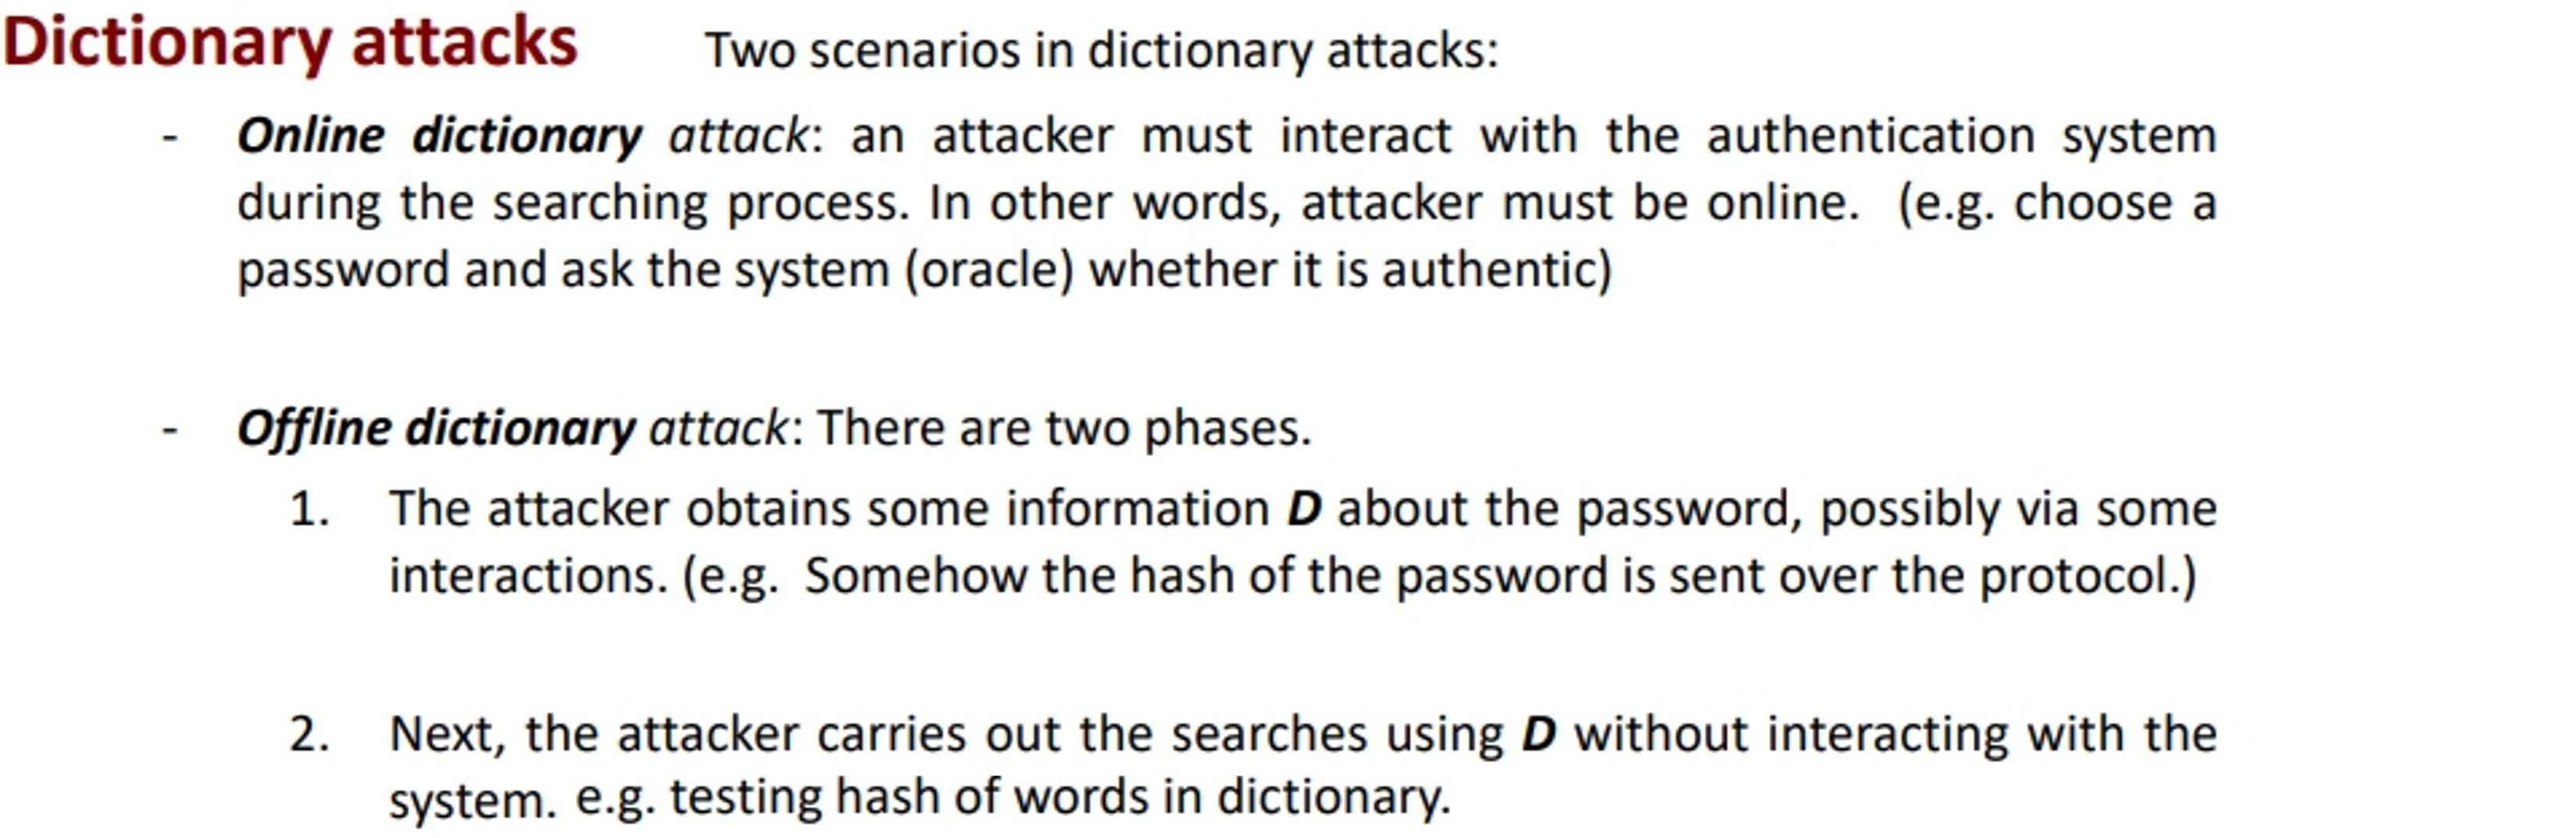
\includegraphics[width=0.95\linewidth]{dictionaryAttack}}

\begin{itemize}
\item \textbf{Stealing of password}: 
\begin{enumerate}
\item \textbf{Sniffing}: Shoulder surfing (look-over-shoulder attack), Sniffing communication (uncommon now, sniffing unencrypted password over public network in clear).
\item \textbf{Viruses, Keylogger}: Computer viruses as key-loggers, or hardware keyloggers. Send captured data back to attack via "covert channel".
\item \textbf{Phishing}: Trick to voluntarily send password to attacker. Social engineering attack. \\
- \textbf{Spear Phishing}: targeted attack against particular small group of users. \\
- \textbf{Phishing, Pharming, Vishing, Smishing} \\
- \textbf{Prevention}: User training, blacklisting.
\item \textbf{Cache}: Shared workstation where information is cached.
\item Lost of password file
\end{enumerate}
\end{itemize}

\subsubsection{Password Strength}
\begin{itemize}
\item \textbf{Password Entropy}: Measure of (randomness) password strength. 
\end{itemize}
\centerline{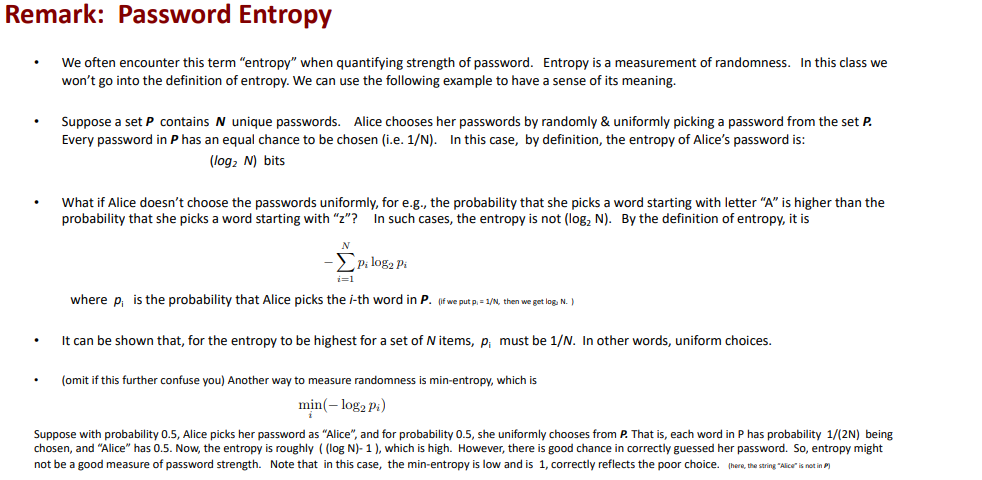
\includegraphics[width=1\linewidth]{passwordEntropy}}
\begin{itemize}
\item Truly random password high "entropy", difficult to remember. User selection biased. Human generated 20-digit password likely to attain 
entropy much less than 20 $log_2(10)$.
\item RFC 4086 suggests password at least 29 bits of entropy to secure against \textbf{online attacks}.
\item If cryptographic keys generated from password, \textbf{offline attacks} possible, password should have at least 128 bits of entropy.
\end{itemize}


\begin{itemize}
\item \textbf{Online vs. Offline attack}: Need to communicate with server not under control to check whether password is correct.
\item E.g. WPA2 personal vulnerable to offline dict. attack. Some "hash" of password sent in clear.
\item \textbf{Enhance password system}: \\
- Make online attack difficult by adding intentional delay / lock. \\
- Make offline attack difficult by applying KDF to password. \\
- System check for weak password / regular changes of password.
\item \textbf{Password vs. Secret Key}: \\
- KDF: key derivation function. \\
- Password as source for crypto secret key. \\
- Using cryptographic hash, hash multiple times to form key, increase cost of exhaustive search. Tradeoff utility.
\end{itemize}

\columnbreak
\begin{itemize}
\item \textbf{Password Files}: \\
\textbf{Hashing}: \\
- File stores userid, password. Add additional layer of protection. \\
- Password file should be "hashed" and "salted"! \\
- (Not "encrypted", don't want way to decrypt and get back) \\
- To authenticate, store and compare hash. \\
\textbf{Salt:} \\
- Need same password hash to two diff. values, for two diff. userid. \\
- (Rainbow table: precomputed table caching outputs of crypto hash function to crack hashes) \\
- Achieve this by salting. New salt randomly generated, concat to pw., output different hash. Salt and hash stored in database.
\end{itemize}

\subsubsection{ATM Skimming}
\begin{itemize}
\item Demonstrates password stealing.
\item Authentication: User presents card, and PIN.
\item Data encoded into magnetic strip using well-known standards, easy to "copy" card by reading and writing to spoofed card.
\item ATM Skimmer: card-reader, camera overlooking keypad / spoofed keypad, some means to record, transmit.
\item \textbf{Measures}: Anti-skimmer devices, shielding keypad, increase awareness, change to unforgeable smartcard.
\end{itemize}

\subsection{2.2 Biometric}
\begin{itemize}
\item \textbf{Biometric data as password}. For identification, or verification.
\item \textbf{Enrollment}: template of user biometric data captured, stored (bootstrapping). \textbf{Verification}: capture biometric data, compare using matching algorithm.
\item Inevitable noise capturing biom. data, leading to error in matching. \\
- \textbf{FMR (False Match Rate)}, \textbf{FNMR (False non-match rate)}. \\
- Adjust threshold to adjust FMR \& FNMR. \\
- \textbf{EER} (Equal Error Rate, FNMR = FMR) \\
- \textbf{FER} (False-to-enroll rate, users' data uncaptureable, e.g. injury)  \\
- \textbf{FTC} (Failure to capture rate, uncaptureable during auth, e.g. finger dirty
\end{itemize}
\centerline{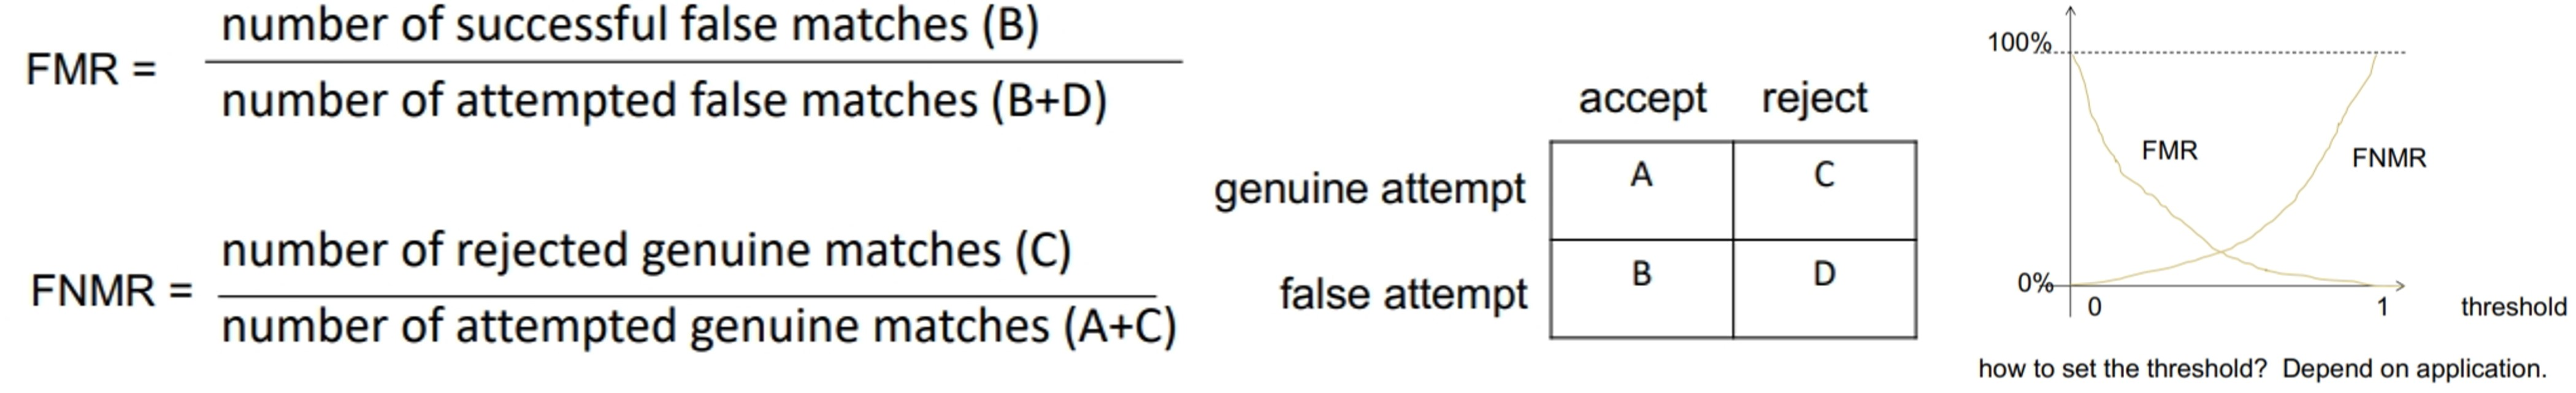
\includegraphics[width=1\linewidth]{FMR}}
\begin{itemize}
\item \textbf{Fingerprint as biometric}: performance depends on quality of scanner, EER range from 0.5\% to 5\%.
\item Biometric data easily spoofable, include \textit{liveness detection} to verify entity.
\end{itemize}

\subsection{2.3 Multi-factor / Multi-step Authentication}
\begin{itemize}
\item \textbf{n-factor Authentication}: Require $n$ authentication factors.
\item \textbf{"Factors"}: \textbf{Know} (Pw, PIN), \textbf{Have} (card, phone, token), \textbf{Are} (Biometric).
\item Must be distinct factors for multi-factor (Know + Have, Have + Are) etc.
\item One Time Password token: \textbf{Time-based /or Sequence-based}.
\item \textbf{2-Step Verification}: Both same factor, e.g (email + password, both "what-you-know", cannot be called "2-factor".)
\item \textbf{out-of-band}: In 2-step verification, two communication channels, main and separate for add. authentication. Non-main called "out-of-band" channel, assume attacker unable to compromise both channels.
\end{itemize}



\columnbreak

\section{3. Authenticity (Data Origin)}

\subsection{Crypto Primitive: Public Key Cryptography}
Public key crypto primitive includes public key encryption and signature. Goal is for confidentiality, and authenticity.
\begin{itemize}
\item Symmetric-key encryption uses same key for encrypt, decrypt.
\item \textbf{Public Key (Asymmetric-key) scheme}: Uses different keys for encryption and decryption.
\item Decryption algo also needs public key. When said "using private key to decrypt", this means using both.
\end{itemize}
\centerline{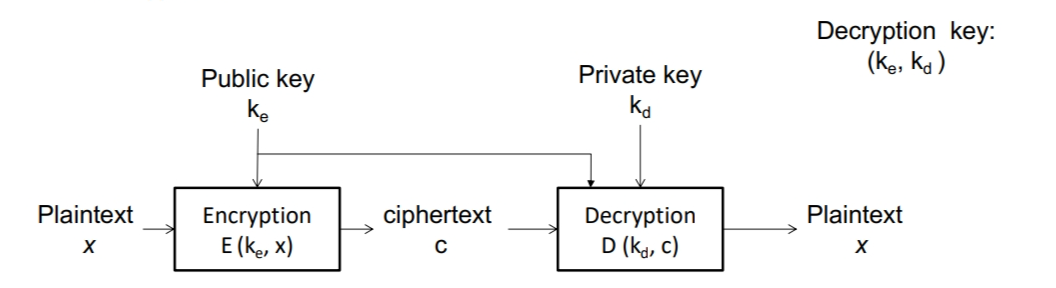
\includegraphics[width=1\linewidth]{publicKeyCrypto}}

\begin{itemize}
\item \textbf{Security Requirement}: Given public key \& ciphertext, difficult to determine private key \& plaintext. (Encryption oracle accessible.)
\item \textbf{(PKC) Public Key Crypto}: Handles scenario of sharing symmetric key via secure channel. PKC only requires secure broadcast channel to distribute the public key. However, building secure broadcast channel to distribute public key is challenging.
\item \textbf{PKC:} Useful for encryption, important application is in authentication (e.g. HTTPS). Limitations compared to symmetric in speed.
\end{itemize}
\centerline{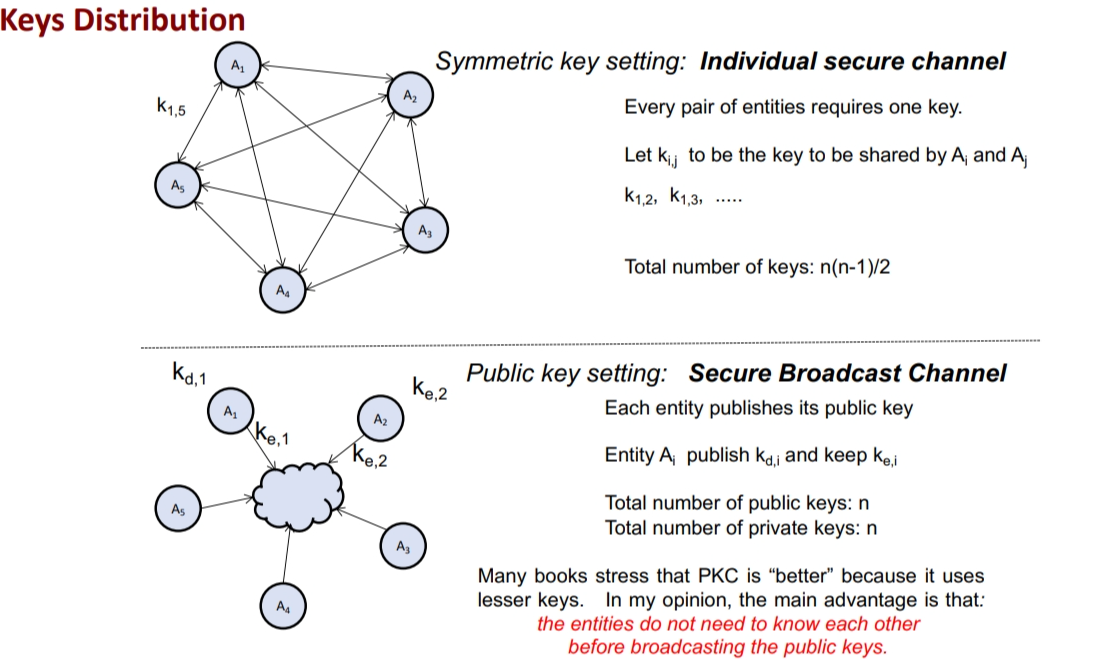
\includegraphics[width=1\linewidth]{keyDistribution}}
\begin{itemize}
\item \textbf{Remark}: Many PKC represent data as integers, algo used are some arithmetic operation on integers, represented using binary.
\item A 1024-bit key is represented under binary representation. An algorithm exhaustively searches 1024-bit integers ($2^{1024}$) is infeasible.
\item For this course, we will consider \textbf{"classroom" RSA}, most basic form RSA.
\item \textbf{In Practice}: Padded RSA (to destroy some property), choose strong primes, fast secure ways to generate primes, secure implementation to guard against side-channel attack, "e" is fixed mostly at 65537. Considerations of quantum computer.
\end{itemize}

\subsubsection{Popular PKC Schemes}
\textbf{RSA}: Key size - 2048 bits. \\
\textbf{ElGamal}: Exploit techniques in Elliptic Curve Cryptography (ECC), reduce key size to - 300 bits. \\
\textbf{Paillier}: Partial homomorphic with respect to addition.



\subsection{Public Key: RSA ("Classroom RSA")}
\centerline{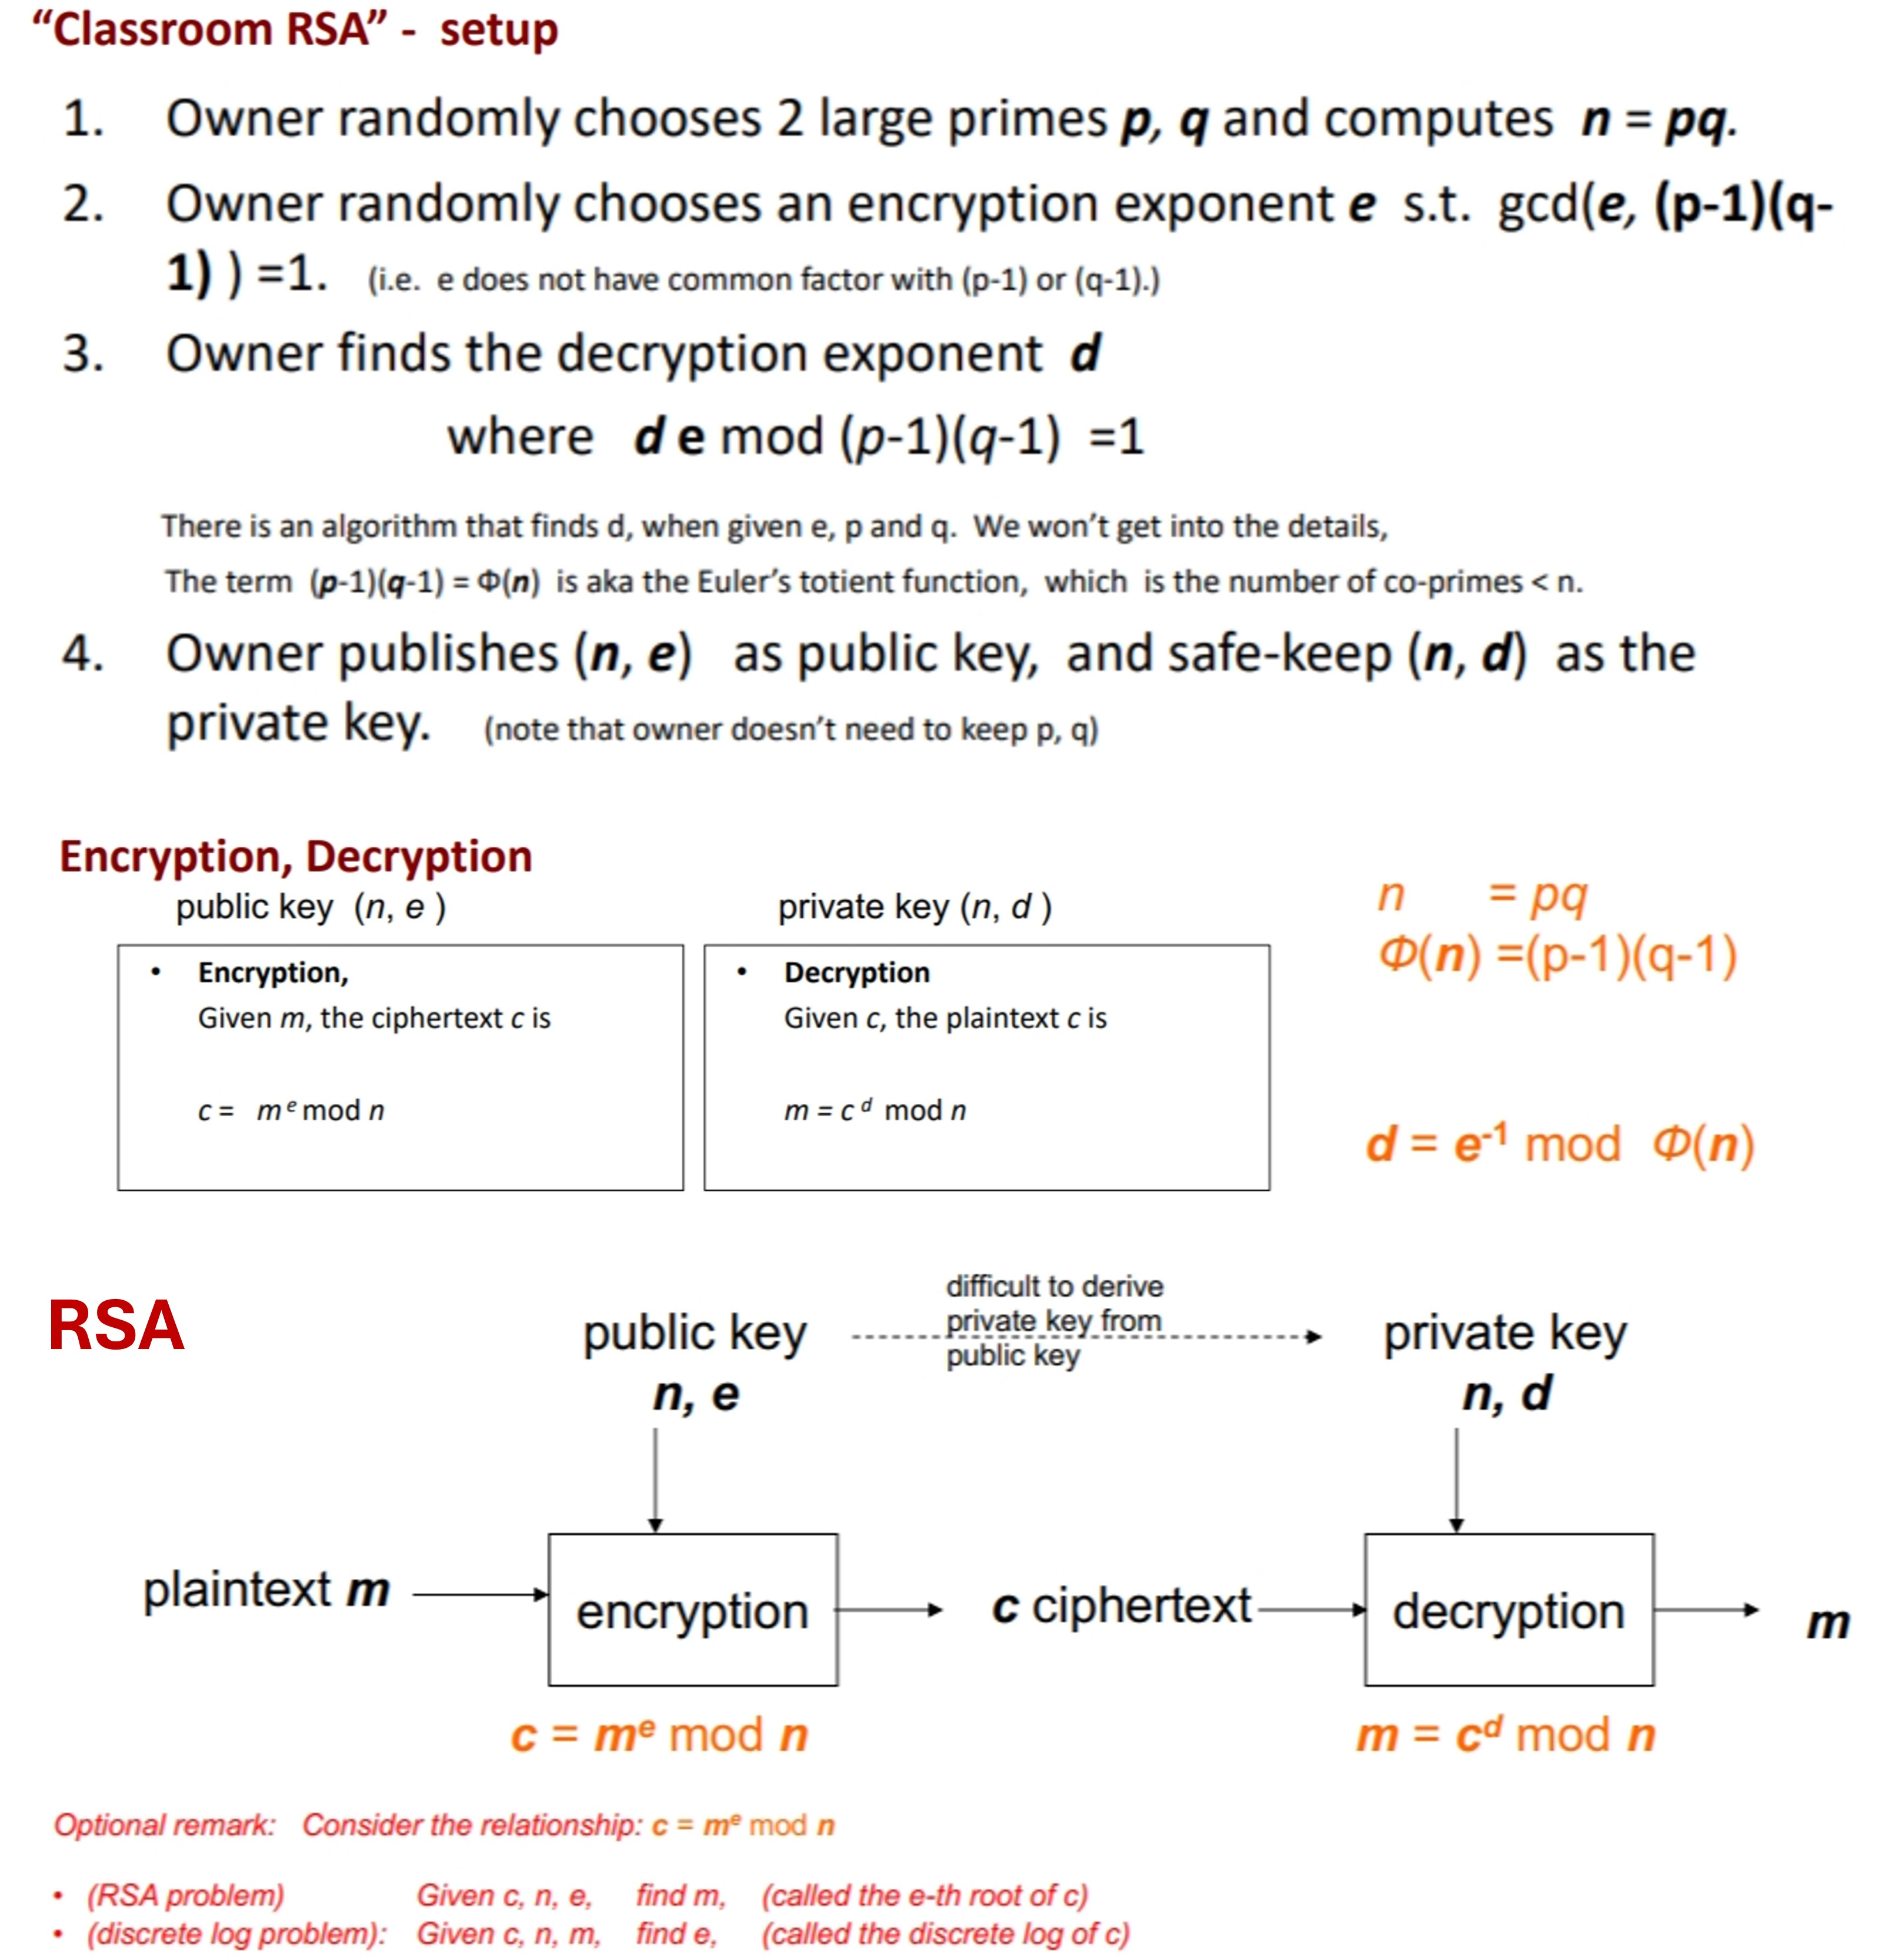
\includegraphics[width=1\linewidth]{classroomRSA}}
\begin{itemize}
\item \textbf{Correctness of RSA}: For any positive $m < n$, and any pair of public/private keys, that \textbf{Decrypt(Encrypt($m$)) = $m$}.
\item $(m^e)^d$ mod $n$ = $m$
\item Correctness depends on the property of modulo.
\end{itemize}
\centerline{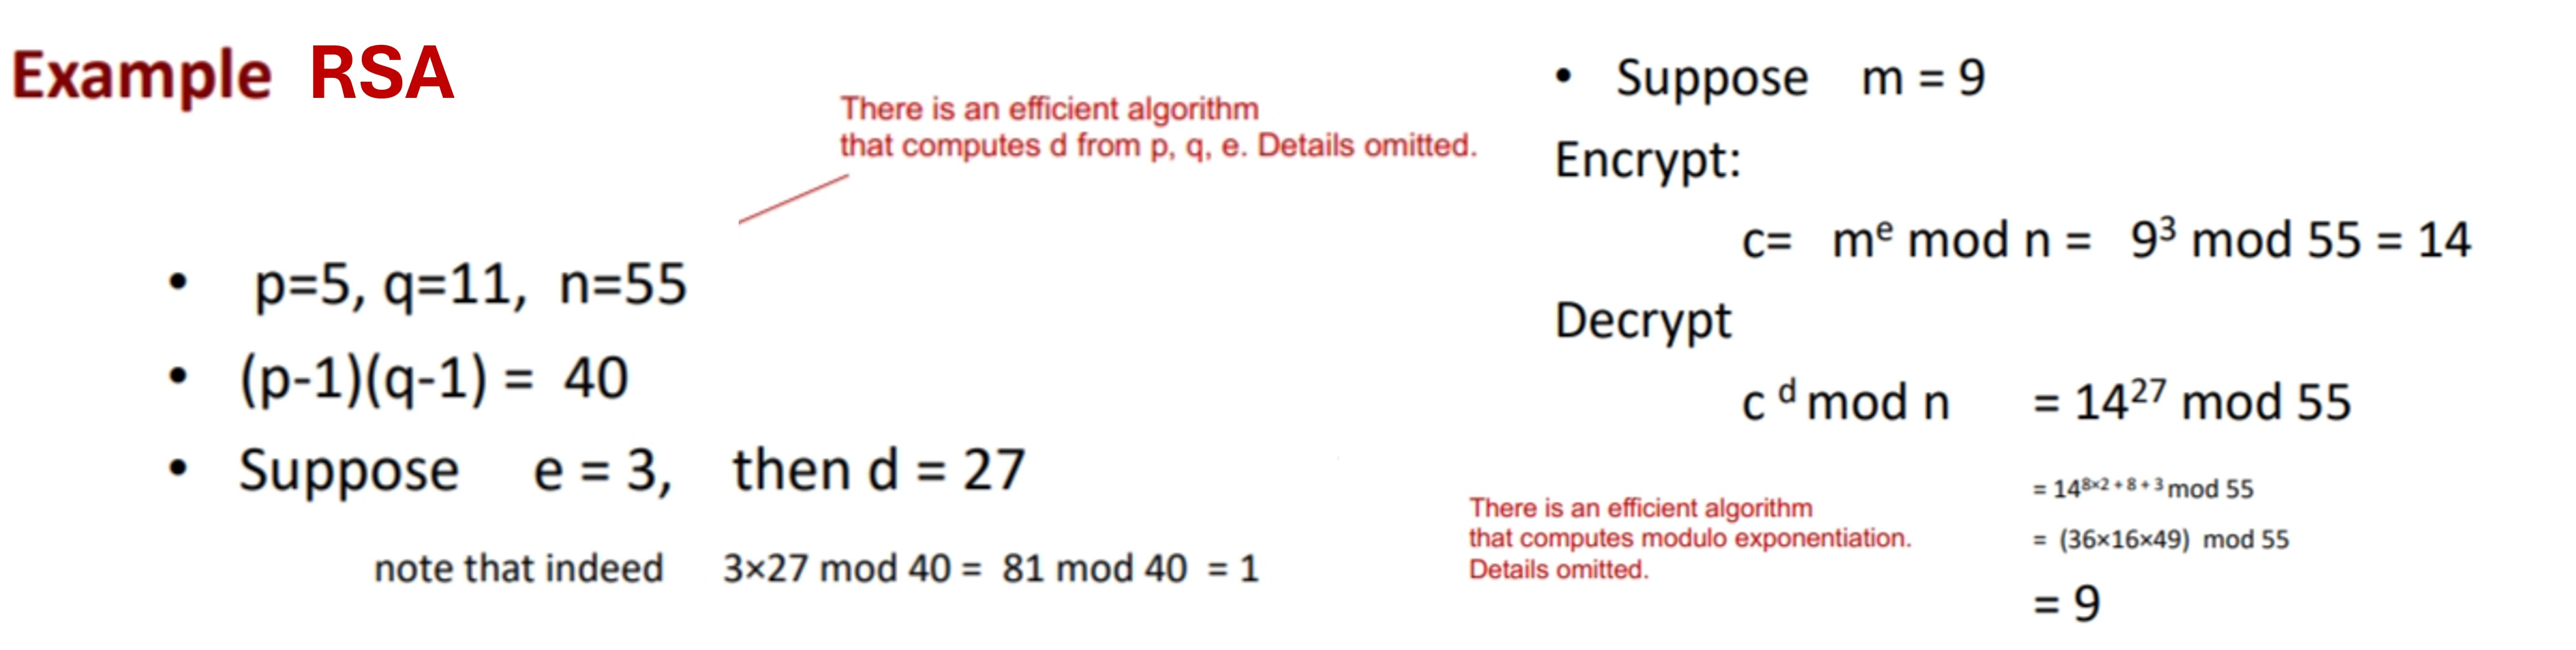
\includegraphics[width=0.9\linewidth]{RSAexample}}
\begin{itemize}
\item \textbf{Interchangeable role of encryption \& decryption key}: Swap role of $d$ and $e$, public can decrypt, owner can encrypt. Usually does not hld in other PKC. This property useful in designing \textbf{signature scheme}.
\item \textbf{Algorithmic Issues}: There is efficient algo to compute exponentiation, hence, efficient way to encrypt, and decrypt (given $n, m, e$, find $m^e$ mod $n$ for encrypt, given $c, d, n$, computer $c^d$ mod $n$).
\item \textit{Step 1 setup}:  Find random prime, randomly pick number, test if prime. (Primality Test). 
\textit{Step 3 setup}: Value of $d$ efficiently computable from $e$ and $n$ using \textit{extended Euclidean algorithm}.
\end{itemize}

\subsubsection{Security of RSA}
\begin{itemize}
\item Getting RSA private key from public key as difficult as factorizing $n$.
\item However, not known whether the problem of getting plaintext from ciphertext as difficult as factorization.
\item \textbf{post-Quantum cryptography}: Generally refers to PKC that are secure against quantum computer.
\item Significant efforts to migrate current systems to post-quantum crypto (Quantum possibility to render RSA algo insecure by 2030). From 2016, NIST plans to choose standard by 2024. Four candidates for Rd 4 (2022). 
\end{itemize}

\subsection{Data Authenticity (Hash): Unkeyed Hash}

\subsection{Data Authenticity (Mac): Keyed Hash}

\subsection{Data Authenticity (Signature): Asymmetric Key}

\subsection{Attacks \& Pitfalls}

\subsection{Birthday Attack on hash}
\subsection{Design flaw: Using encryption for authenticity}
\subsection{Time-Space tradeoff}






















\end{multicols*}
\end{document}
